
% Copyright 2007, 2008, 2009 Elsevier Ltd 
% 
% This file is part of the 'Elsarticle Bundle'.
% --------------------------------------------- 
%
% It may be distributed under the conditions of the LaTeX Project Public
% License, either version 1.2 of this license or (at your option) any
% later version.  The latest version of this license is in
%    http://www.latex-project.org/lppl.txt
% and version 1.2 or later is part of all distributions of LaTeX
% version 1999/12/01 or later c.
%
% The list of all files belonging to the 'Elsarticle Bundle' is
% given in the file `manifest.txt'.
%
 
% Template article for Elsevier's document class `elsarticle'
% with harvard style bibliographic references
% SP 2008/03/01
%
%
%
% $Id: elsarticle-template-harv.tex 4 2009-10-24 08:22:58Z rishi $
%
%
%\documentclass[preprint,authoryear,12pt]{elsarticle}
\documentclass[preprint,12pt]{elsarticle}

% Use the option review to obtain double line spacing
%\documentclass[authoryear,preprint,review,12pt]{elsarticle}

% Use the options 1p,twocolumn; 3p; 3p,twocolumn; 5p; or 5p,twocolumn
% for a journal layout:
%\documentclass[final,authoryear,1p,times]{elsarticle}
%\documentclass[final,authoryear,1p,times,twocolumn]{elsarticle}
%\documentclass[final,authoryear,3p,times]{elsarticle}
%\documentclass[final,authoryear,3p,times,twocolumn]{elsarticle}
%\documentclass[final,authoryear,5p,times]{elsarticle}
%\documentclass[final,authoryear,5p,times,twocolumn]{elsarticle}

%% if you use PostScript figures in your article
%% use the gra

%%graphis package for simple commands
%% \usepackage{graphics}
%\usepackage{cases}
%% or use the graphicx package for more complicated commands
\usepackage{graphicx}
%% or use the epsfig package if you prefer to use the old commands
\usepackage{epsfig}
%\usepackage{subfig}
\usepackage{comment}

\usepackage{epstopdf}
\usepackage{pdflscape}
\usepackage{bm}
\usepackage{hyperref,url}
\hypersetup{colorlinks=true, urlcolor=blue, linkcolor=blue, citecolor=red}

%% The amssymb package provides various useful mathematical symbols

\usepackage{amssymb,amsmath,array}
%The amsthm package provides extended theorem environments

\usepackage{amsthm}
\usepackage{graphicx}
%\usepackage{subfigure}
  
%% The lineno packages adds line numbers. Start line numbering with
%% \begin{linenumbers}, end it with \end{linenumbers}. Or switch it on
%% for the whole article with \linenumbers after \end{frontmatter}.
%% \usepackage{lineno}

\usepackage{lscape}

%% natbib.sty is loaded by default. However, natbib options can be
%% provided with \biboptions{...} command. Following options are
%% valid:

%%   round  -  round parentheses are used (default)
%%   square -  square brackets are used   [option]
%%   curly  -  curly braces are used      {option}
%%   angle  -  angle brackets are used    <option>
%%   semicolon  -  multiple citations separated by semi-colon (default)
%%   colon  - same as semicolon, an earlier confusion
%%   comma  -  separated by comma
%%   authoryear - selects author-year citations (default)
%%   numbers-  selects numerical citations
%%   super  -  numerical citations as superscripts
%%   sort   -  sorts multiple citations according to order in ref. list
%%   sort&compress   -  like sort, but also compresses numerical citations
%%   compress - compresses without sorting
%%   longnamesfirst  -  makes first citation full author list
%%
%% \biboptions{longnamesfirst,comma}

% \biboptions{}

\newcommand{\JGnote}[1]{\fbox{\parbox{\textwidth}{ \color{red} JG Note $\Rightarrow$ #1}}}
\newcommand{\BLnote}[1]{\fbox{\parbox{\textwidth}{ \color{green} BL Note $\Rightarrow$ #1}}}
\newcommand{\red}{\textcolor{red}}
\newcommand{\blue}{\textcolor{blue}}
\newcommand{\green}{\textcolor{green}}
\newcommand{\frc}{\displaystyle\frac}
\newcommand{\PN}[2][error]{P$_{#1}$DG-P$_{#2}$}
\newcommand{\PNDG}[2][error]{P$_{#1}$DG-P$_{#2}$DG}
\newcommand{\eg}{{\it e.g., }} 
\newcommand{\ie}{{\it i.e., }}

\journal{Applied Mathematical Modelling}

\begin{document}

\begin{frontmatter}

%% Title, authors and addresses

%% use the tnoteref command within \title for footnotes;
%% use the tnotetext command for the associated footnote;
%% use the fnref command within \author or \address for footnotes;
%% use the fntext command for the associated footnote;
%% use the corref command within \author for corresponding author footnotes;
%% use the cortext command for the associated footnote;
%% use the ead command for the email address,
%% and the form \ead[url] for the home page:
%%
%% \title{Title\tnoteref{label1}}
%% \tnotetext[label1]{}
%% \author{Name\corref{cor1}\fnref{label2}}
%% \ead{email address}
%% \ead[url]{home page}
%% \fntext[label2]{}
%% \cortext[cor1]{}
%% \address{Address\fnref{label3}} 
%% \fntext[label3]{}

\title{A Reduced Order Model for Permeability Fields Using Singular Value Decomposition, SVD, by Interpolating in the Principal Component Spaces \red{(Maybe you should consider a shorter and punchier title ...)}}
\author[UoA]{B. Lashore\corref{cor1}}\ead{lashorebabatunde@yahoo.com} \author[UoA]{J.L.M.A. Gomes} \author[UoA]{K. Christou}
\cortext[cor1]{Corresponding author.}
\address[UoA]{Mechanics of Fluids, Soils \& Structures Research Group \\ School of Engineering University of Aberdeen, UK}


\begin{abstract}
Nice Abstract - Short, punchy
\\
\\
\\
\\
\\
\\ 
\end{abstract}



\begin{keyword} %% keywords here, in the form: keyword \sep keyword
Singular Value Decomposition, SVD\sep Upscaling\sep Model Order Reduction, MOD \sep  Principal Component Spaces \sep Permeability field
\end{keyword}
 
\end{frontmatter}

%%%%%%%%%%%%%%%%%%%%%%%%%%%%%%%%%%%%%%%%%%%%%%%%%%%%%%%%%%%%%%%%%%%%%%%%%%%%%%%%%%%%%%%%%%%%%%%%%%%%%%%%%%%%%%%%%%%%%%%%%%%%%%%%%%%%%%%%%%%%%%%%%%%%%%%%%%%%%%%%%%%%%%%%%%%%%%%%%%%%%%%%%%%%%%%%%%% 
\section{Introduction}\label{section:intro}
Naturally occuring rock formations are inherently heterogeneous, which means that rock properties such as permeability, pore spaces ({\it i.e.}, porosity) and pore throat vary spatially at different length scales. The heterogeneity of rock formations (\ie porous media) is relevant in calculations of transport and storage of fluids in porous media. Therefore, the representation of these heterogeneous properties is of great importance to oil and gas (\ie reservoir management), carbon capture and storage (CCS, \ie CO$_2$ transportation and storage in subsurface rocks) and waste management (\ie remediation of contaminated soil).

\JGnote{You need to ensure that the paragraphs are somehow linked ... \eg how is the first sentence of the following paragraph linked with the previous paragraph? }

Furthermore, due to limitations in computing resources, for simulations with very fine grids it is neither efficient nor possible to obtain exact values of geological properties at all spatial coordinates of the domain (\ie scale problems) \cite{chen_2006,miller_1998,Renard_1997}. This is particularly true for large geological domains which span several kilometres. Additionally, it is not possible to obtain reliable and accurate spatial information about geological properties throughout the domain ({\it i.e.}, uncertainty problems) \red{(Isn't this sentence a repetition of the first one?)}. It is possible to overcome these challenges by upscaling. Upscaling techniques solve both problems by replacing discrete geological and fluid properties of detailed high resolution domains with coarse descriptions (low resolution) of these properties \cite{Vereecken_2007}.

Upscaling techniques which best preserve the statistical properties and flow dynamics behaviour of the high resolution domain give the best representation of the heterogeneous property. There are several upscaling techniques which fall under different categories \cite{Hasting_2001, Renard_1997, Szymkiewicz_2013}, however over the last decade, techniques classed as stochastic have received great attention from academic and industrial porous media communities worldwide \cite{Guilleminot_2012, Ravalec-Dupin_2010, Verwoerd_2009}. One of the reasons for this is because stochastic techniques are robust enough to handle multiphase flow in porous media, and they address scale and uncertainity problems which were previously mentioned.

\JGnote{The technique we are using/advocating here is not stochastic, though it would be good to develop it further, \ie brief lit review. Maybe you should add a few sentences/paragraphs on: ROM and the use of SVD for upscalling ... }
\medskip

This work couples stochastic and deterministic upscaling representations of the permeability field to a novel high-order accurate control volume finite element method (CVFEM) (see \cite{Gomes_2017} for further details of the model formulation) so as to investigate statistical properties and multiphase flow behaviour in highly heterogeneous porous media. \red{(Try to split this really long sentence ...)} 

Four upscaling techniques are investigated in this work. Arithmetic and harmonic means are used to obtain the first two upscaled representation and these two are classed as deterministic techniques. The third is a randomly generated permeability field with a Gaussian distribution, prescribed by a probability density function (PDF) which was obtained from a domain discretised with high-resolution mesh with known permeability distribution (\ie  base case). The fourth upscaling technique is the crux of this research, it introduces singular value decomposition (SVD) as a method of upscaling using interpolation within the concept of principal component space to reduce the order of the permeability field \red{(Sentence is quite confusing and does not say much ...)}.

In Section 2, the basic mathematical explanation of SVD and its associated properties are presented. Then, the concept of spaces is explained from the engineer's perspective and also from the mathematician's perspective. The objective of this explanation is to assist both parties in visualizing the relevant spaces and performing the necessary transformation within those spaces. Finally, the section describes model order space reduction for the permeability field within the principal component space. Section 3, starts by describing the high resolution base case on which the four upscaling techniques are modelled. The the simulation run which is similar for all the cases/models is described. A brief summary of the pre-processing step for each of the models is also presented. Section 4 provides the results and some discussion on the results of the simulations. It als gives further intepretation to the result obtained from the SVD upscaling technique. Finally, section 5 provides the conclusion.


\section{Singular Value Decomposition, SVD, and its application for reducing the order of a permeability field}\label{section:svd}
\subsection{A Brief Introduction to SVD}\label{subsection:svd_brief}

Singular Value Decomposition, SVD, \JGnote{ioioioiok} exists within the linear algebra branch of mathematics as one of the most exciting means of factorizing a matrix, $\mathbf{A}$, into three parts $\mathbf{U}$, $\Sigma$ and $\mathbf{V}$. Where $\mathbf{U}$ and $\mathbf{V}$ are orthonormal, and $\Sigma$ is a diagonal matrix. If $\mathbf{A}$, is a square matrix then $\mathbf{U}$, $\Sigma$ and $\mathbf{V}$ are square matrix and $\mathbf{U}^{\intercal}\mathbf{U} = \mathbf{V}^{\intercal}\mathbf{V} = \mathbf{I}$. But if $\mathbf{A}$ is an $m * n$ matrix, $\mathbf{U}$ and $\mathbf{V}$ still remain as square matrices, albeit with different matricial sizes. $\mathbf{U}$ is an $m * m$ while $\mathbf{V}$ is an $n * n$. Another interesting property of $\mathbf{U}$ and $\mathbf{V}$ since they are square (irrespective of whether A is square or rectangular) is that $\mathbf{U}^{-1} = \mathbf{U}^{\intercal}$ and $\mathbf{V}^{-1} = \mathbf{V}^{\intercal}$. When $\mathbf{A}$ is an $m * n$ matrix, $\Sigma$ is a diagonal $m x n$ matrix. The diagonal entries of $\Sigma$ (in both the case of square and rectangular matrices) are referred to as the singular values of $\mathbf{A}$, and are usually denoted by sigma ($\sigma_{1}, \sigma_{2},..., \sigma_{r}$). For a rectangular matrix, the singular values fill the first $r$ places on the main diagonal of $\Sigma$, where $r$ is the rank of A. Additionally, the $i$th singular value, $\sigma_{i}$ is ordered such that $\sigma_{1} \geq \sigma_{2} \geq ...\geq \sigma_{r}$. A huge benefit of the SVD is the orthogonality of the columns in $\mathbf{U}$ and $\mathbf{V}$. The columns of $\mathbf{U}$ are known as the left singular vectors while the columns in $\mathbf{V}$ are known as the right singular vectors. A simple consideration of the benefit of this, is the ease with which it allows the inverse of square matrix $\mathbf{A}$ to be calculated. This example is presented thus:

\begin{equation}
 \mathbf{A}x = b
\end{equation}
\begin{equation}
 \mathbf{U} \Sigma \mathbf{V}^{\intercal} x = b
\end{equation}
\begin{equation}
 x = \mathbf{V} \Sigma^{-1} \mathbf{U}^{\intercal} b
\end{equation}

\subsection{Principal Component Spaces and Model Order Reduction for the permeability field}\label{subsection:pcspaces}

\subsubsection{Visualizing the permeability space}\label{subsubsection:visualization_permspace}
In real-life ({\it i.e.}, a 3D geometry), permeability is a tensor quantity, but for the purpose of the following explanation (and the remaining part of this paper), a 2D geometry is assumed where permeability is a scalar quantity. Furthermore, the simulator prescribes the permeability field using $P0DG$ element type, which means that permeability values are assigned in the middle node of the triangular unstructured mesh used for discretizing the 2D simulation geometry. And the value assigned in the middle node of the triangle represents the permeability value for the whole triangular element. But for simplicity, in the remaining part of this section, we will imagine or assume the $2D$ geometry is discritized by a square grid with the value for each square element assigned in the middle of the element. This explanation allow one to easily visualize this permeability space because it is defined by the $x,y$ co-ordinates  system which most people are already familiar with. The model order reduction for the permeability field discussed here is concerned with reducing the volume of permeability data within the permeability space. Consider for instance a small square which is discretized to contain four squares such that $4$ data values are defined in the middle of the four squares. The permeability space of $4$ can be reduced to a smaller value of $1$ through an averaging process such as arithmetic, harmonic or geometric mean. This type of reduction is the focus of this paper, albeit the main focus of this paper is achieving this reduction through singular value decomposition in the principal component spaces. 

\subsubsection{Visualizing the principal component spaces}\label{subsubsection:visualization_pcspaces}
Essentially, the existing permeability space is transformed through SVD to principal component spaces where usually, traditional principal component analysis is performed before interpolation is used to implement further data reduction in the principal component spaces. This reduced data in the principal component space is then transformed back into the permeability space to obtain a reduced permeability space.

The principal component space is a bit more challenging to visualize because it usually consists of more than $3$ dimensions. $3D$ ({\it i.e.}, $x, y$ and $z$ in the cartesian plane) being the natural dimension which humans exist, is easy to visualize. Many engineers are also able to visualize 4D with time as the fourth dimension, albeit only few scientists and engineers are able to visualize and work in the abstract dimension where the number of dimensions exceed four. An aid for visualizing the PC space is to write out the $\mathbf{U}$, $\mathbf{\Sigma}$ and $\mathbf{V^{\intercal}}$ matrices (or imagine the matrices written out) and consider the singular vectors ({\it i.e.},columns in $\mathbf{U}$ and rows in $\mathbf{U}$) as separate principal component spaces.

\subsubsection{Model Order Reduction/Principal Component Space Reduction}\label{subsubsection:svdcase_preprocess_algorithm}
 For the SVD model order reduction of the permeability field, all the work is done in the principal component spaces. This can be completed in two steps. The first step is optional and it is the well known principal component analysis (PCA). Here, the singular values are examined and based on a pre-defined criteria, z singular values are selected, starting from $\sigma_{1}$ and in a decreasing order. $z \leq r$, where in the case $z = r$, it can be assumed that step 1 has been ignored. In the case where $z < r$, the first z columns of $\mathbf{U}$ and the first z rows of $\mathbf{V^{\intercal}}$ are extracted from $\mathbf{U}$ and $\mathbf{V^{\intercal}}$ to form new matrices $\mathbf{U_{new}}$ and $\mathbf{V^{\intercal}_{new}}$ respectively. The selected z singular values also for a new diagonal matrix ({\it i.e.}, where $z < r$).

The second step involves interpolation within each singular vector (column in $\mathbf{U}$ and row in $\mathbf{V^{\intercal}}$), to reduce the number of data in each column of  $\mathbf{U}$ and in $\mathbf{V^{\intercal}}$. From this step,  $\mathbf{U_{new2}}$ and $\mathbf{V^{\intercal}_{new2}}$ are obtained. The reduced permeability field is calculated by multiplying  $\mathbf{U_{new2}}$ $\mathbf{\Sigma_{new}}$ and $\mathbf{V^{\intercal}_{new2}}$. 

\section{Brief Overview of Upscaling}\label{section:overview_upscaling}

The first section briefly introduced the rational behind upscaling. This is a subject which has interested the academic community for over $7$ decades.  \citet{Cardwell_1945} investigated arithmetic and weighted averages as upscaling techniques for calculating a single equivalent permeability for an oil reservoir with varying permeabilities. \citet{King1996} investigated the use of renormalization for upscaling. And \citet{Yeo2001} discussed the accuracy of renormalization method for upscaling 2 dimension hydraulic conductivity fields.  \citet{Renard_1997} provided a comprehensive review of the various techniques for upscaling in \citeyear{Renard_1997}. \citet{Christie_2001SPE10Model} provided $2$ sets of problems to compare the upscaling and upgridding techniques of different simulators.

\section{Model Description and Simulation Setup}\label{section:model_simulation}

\subsection{Model Description}\label{subsection:model}
The BaseCase  ({\it i.e.} fine resolution) model for the permeabiliy field builds on the $2 * 2$ block, $4$ quadrant model used initially by \citet{Cardwell_1945} and later by \citet{Yeo2001} and \citet{dawe_2008}. These authors designed the permeability field for the quadrants in a checkerboard style which means that diagonally opposite blocks retained the same permeability values with one set of diagonally opposite blocks having a higher permeability value compared to the other se. So that, one set of diagonally opposite blocks are referred to as high permeability blocks while the other set is referred to as low permeability blocks. The BaseCase permeability model used in this manuscript retains the checkerboard desgined used by the recently named authors. Albeit, the permeability data for each block in the set of diagonally opposite blocks have similar value ({\it i.e.} not exactly the same as in the papers referred to), although one set can still be referred to as a set of high permeability blocks while the other set is referred to as a set of low permeability blocks. Futhermore, within each block, the permeability field varies within a predefined range and consists of $1600$ permeability values. More details on the design of the permeability field for the BaseCase is available in section~\ref{subsubsection:basecase_preprocess_algorithm}. And Fig.~\ref{fig:PermFields}a and~\ref{fig:PermFields}b give a pictorial representation of the permeability field for the base case with the mesh discretization visible and invisible respectively. Using the labelling scheme used by \citet{dawe_2008}, the quadrant model block $K1, K2, K3$ and $K4$ are top left, bottom left, top right and bottom right respectively.

Four upscaled permeability field models were obtained from the high-resolution ({\it i.e.} the BaseCase) permeability field. And compared to the BaseCase model, all the upscaled models were upgridded to reduce the resolution of the permeability field. Specifically, for the simulation domain, the high resolution ({\it i.e.} BaseCase) model had 4112 triangular elements while the upscaled models had 728 triangular elements. The first two upscaled models are referred to as the ArithMean and the HarmMean Case, and this is because they are based on the arithmetic and the harmonic averaging methods, respectively. In both the ArithMean and HarmMean Cases, averages are calculated for each block using the $1600$ data points from the blocks of the BaseCase to obtain a permeability value for each block in the upscaled models. This effectively homogenizes the permeability field in each block. The upscaled permeability field for the third and fourth cases are referred to as PDFCase and SVDCase, respectively. And, as can be deduced from the names, these cases are based on probability density function (PDF) and singular value decomposition (SVD). The description for these permeability field models are more involved and are presented in section ~\ref{subsubsection:pdfcase_preprocess_algorithm} and ~\ref{subsubsection:svdcase_preprocess_algorithm} respectively. It is appropriate to note that although these models (PDFCase and SVDCase) are upscaled, they retain heterogeneity within the blocks.

\subsubsection{BaseCase Pre-processing Algorithm}\label{subsubsection:basecase_preprocess_algorithm}
\begin{enumerate}[1]
  \item A function is used to randomly generate uniform ({\it i.e.} Gaussian) data for each block. The range for each block is as below:
  \begin{enumerate}[a]
    \item \textbf{K1} :
    \item \textbf{K2} :
    \item \textbf{K3} :
    \item \textbf{K4} : 
  \end{enumerate}                                                    
  \item The number of data generated for each block is $1600$ and the data is randomly position within each block in a structured pattern. Albeit, the simulation grid ({\it i.e.} mesh) is unstructured.
  \item Merge data from different blocks into a single file retaining the original ``structured pattern'' (in step 1 above) for the randomly positioned data in each block. This file will be used by the Control Volume Finite Element Method (CVFEM) simulator to prescribe the permeability field for the base case.
\end{enumerate}


\subsubsection{PDFCase Pre-processing Algorithm}\label{subsubsection:pdfcase_preprocess_algorithm}
\begin{enumerate}[1]
  \item Data from step one of the pre-processing algorithm for the base case is used to calculate the mean and standard deviation for each block of the permeability field.
  \item A function which generates a Gaussian data set using arithmetic mean and standard deviation is used to stochastically produce a quater of the number of data in the base case for each of the four blocks.
  \item The number of data generated for each block is $400$ and the data is randomly position within each block in a structured pattern. As in the base case, the simulation grid ({\it i.e.} mesh) is unstructured.
  \item Finally, the structured data from each block is combined into a single file and then provided to the CVFEM simulator.
\end{enumerate}


\subsubsection{SVDCase Pre-processing Algorithm}\label{subsubsection:svdcase_preprocess_algorithm}
\begin{enumerate}[1]
  \item The permeability field obtained in step 3 of the pre-processing algorithm for the base case is factorized using SVD to obtain $\mathbf{U}, \Sigma,$ and $\mathbf{V}$.
  \item A selected number, $z$, of singular values are retained in decreasing order of magnitude to form a new diagonal matrix, $\Sigma_{new}$.
  \item The first $z$ columns of $\mathbf{U}$ and $\mathbf{V}$ are selected to form new truncated matrices call $\mathbf{U_{new}}$ and $\mathbf{V_{new}}$ respectively.
  \item Within each column of $\mathbf{U}$ and $\mathbf{V}$ a linear interpolation is performed to form a new column with the number of data in each column reduced to a half of the original column. And, these new columns are recombined to form $\mathbf{U_{new2}}$ and $\mathbf{V_{new2}}$.
  \item The permeability field used for the SVD case is the matrix, $\mathbf{A_{new2}}$ which is defined as $\mathbf{U_{new2}} \mathbf{\Sigma_{new}} \mathbf{V_{new2}^{\intercal}}$. It is a permeability field with a quater of the data in the base cased and therefore a permeability field with a reduced order.  
\end{enumerate}

\subsection{Simulations}\label{subsection:simulations}
For the simulations, each of the model's domain is initially fully saturated with a fluid (Phase 2), and a wetting phase (1) fluid is driven into the domain from the left hand side at a constant mass flow rate. Newmann ({\it i.e.} no flux) boundary conditions were imposed on the upper and lower borders of each domain, while mixed fluids are recovered from the right-hand face. Fig (...........)a shows the permeability field of the base case while fig (....... - ........) shows the phase saturation field during fluid injection for time, $t = 0.15s, 0.30s, 0.50s, 1.15s, 1.75s$ and $2.95s$.

\section{Results and Discussion}\label{section:results_discussion}

Talk about those beautiful screenshots!\\
\\
\\
\\
\\
\\
\\
\\
\\
\\
\\
\\
\\
\\
\\
\\
\\
\\
\\
\\
\\
\\
\\
\\
\\
\\
\\
\\
\\
\\
\\

\section{Conclusion}\label{section:conclusion}

Conclude man!\\
\\
\\
\\
\\
\\
\\
\\
\\
\\
\\
\\
\\



%\section{Acknowledgements}
%Mr William Rad\"unz would like to acknowledge the support from the Brazilian Research Council (CNPq) under the \textit{Science without Borders scholarship programme}. Mr Konstantinos Christou would like to acknowledge the support of the University of Aberdeen - College of Physical Science as well as the Aberdeen Formation Evaluation Society (\textit{AFES} is an SPWLA chapter). 

\clearpage 
%% References with bibTeX database:
\bibliographystyle{elsarticle-harv} 
%\bibliographystyle{elsarticle-num}
%\bibliographystyle{apacite}
\bibliography{references}
  
\clearpage 

\listoftables
\clearpage
%
\begin{landscape}
\begin{table}
  \begin{tabular}{c | c c  c  c  c  c  c  c  c  c  c   c}
    \hline
      {\bf Section} & $\phi$ & VR  & $S^{0}_{w}$ & $S^{0}_{nw}$ & $K_{1}$ & $K_{2}$ & $K_{3}$ & $K_{4}$ & $K_{5}$ & $S_{w,irr}$ & $S_{nw,r}$ & $u^{0}_{w}$ \\ 
    \hline
      \ref{section:results_validation} & 0.2  & 1.0  & 0.0  & 1.0  & 1.0  & 2.5  & N/A  & N/A  & N/A & 0.2  & 0.3 & 1.0 \\
      \ref{section:results_homo_hete}   & 0.2  & 1.0  & 0.0  & 1.0  &  XX  & N/A  & N/A  & N/A  & N/A & 0.2  & 0.3 & XX  \\
                                       & 0.2  & 10.0 & 0.0  & 1.0  &  XX  & N/A  & N/A  & N/A  & N/A & 0.2  & 0.3 & XX  \\
      \hline
   \end{tabular}
   \caption{Sumary of model set-up used in the numerical simulations. Superscript $0$ denotes initial condition. \red{(KOSTAS, PLEASE: 1. DOUBLE CHECK THE K, u and S0 VALUES FROM THE MPML FILES; 2. REPLACE ALL XX; 3. COMPLETE THE TABLE FOR ALL SECTIONS/SIMULATIONS.  $S_{w,irr}$ and $S_{nw,r}$ are the same for all simulations.) }}\label{table:setup}
\end{table}
\end{landscape}
\clearpage

\clearpage  
\listoffigures
\clearpage

%%%%
%%%%  FIGURE 
%%%%
\begin{figure}[h]
\centering
\vbox{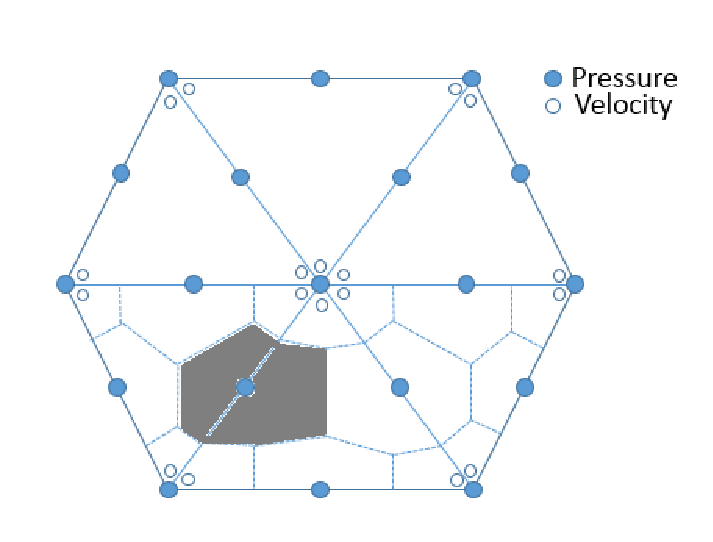
\includegraphics[width=.5\textwidth]{./Pics/P1DGP2.pdf}}
\caption{2D representation of \PN[1]{2} element pairs used in this work. Shaded areas denote control volumes across two contiguous elements. Blue and white circles represent pressure and velocity nodes, respectively.} 
\label{fig:fem_cv}
\end{figure}

\clearpage

%%%%
%%%%  FIGURE
%%%%
\begin{figure}[h]
\centering
\vbox{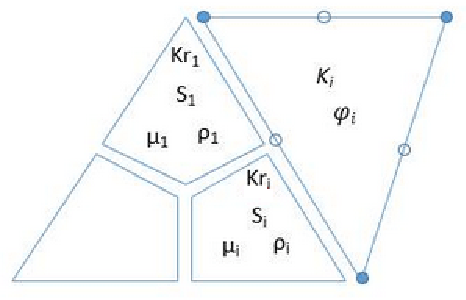
\includegraphics[width=.75\textwidth]{./Pics/element_n.pdf}}
\caption{This is a graphical representation of two different element types. Triangle {\it A} is a representation of the \PN[1]{2} element-pair, whereas triangle {\it B} represents the \PN[1]{1} element-pair. Porosity $\phi_{i}$, permeability {\bf K}$_{i}$, velocity and pressure are primarily represented in FE space whereas scalar fields (such as saturation, density, viscosity etc) are represented in CV space.}
\label{fig:fem_elem}
\end{figure}
\clearpage

%%%%
%%%%  FIGURE 
%%%%
\begin{figure}[h]
\centering
\vbox{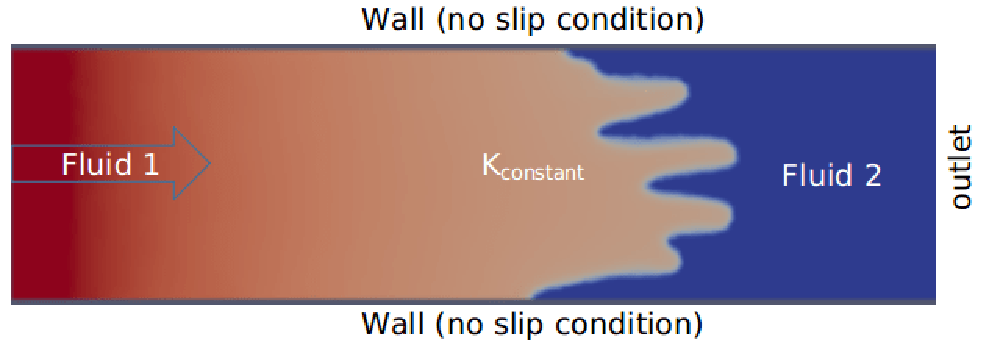
\includegraphics[width=0.75\textwidth]{./Pics/phase_vol_frac_uni_perm_1.pdf}}
\caption{Schematics of formation of flow instabilities during injection of a pure low viscosity fluid (red) into a domain saturated with a second fluid (dark blue). The ratio of viscosity between the two fluids is 5. In this case, the initially piston shape front collapses leading to the formation of several fingers.}
\label{fig:simple_case}
\end{figure}
\clearpage


%%%%
%%%%  FIGURE 
%%%%
\begin{figure}[ht] 
\vbox{
\hbox{\hspace{-0.3cm}
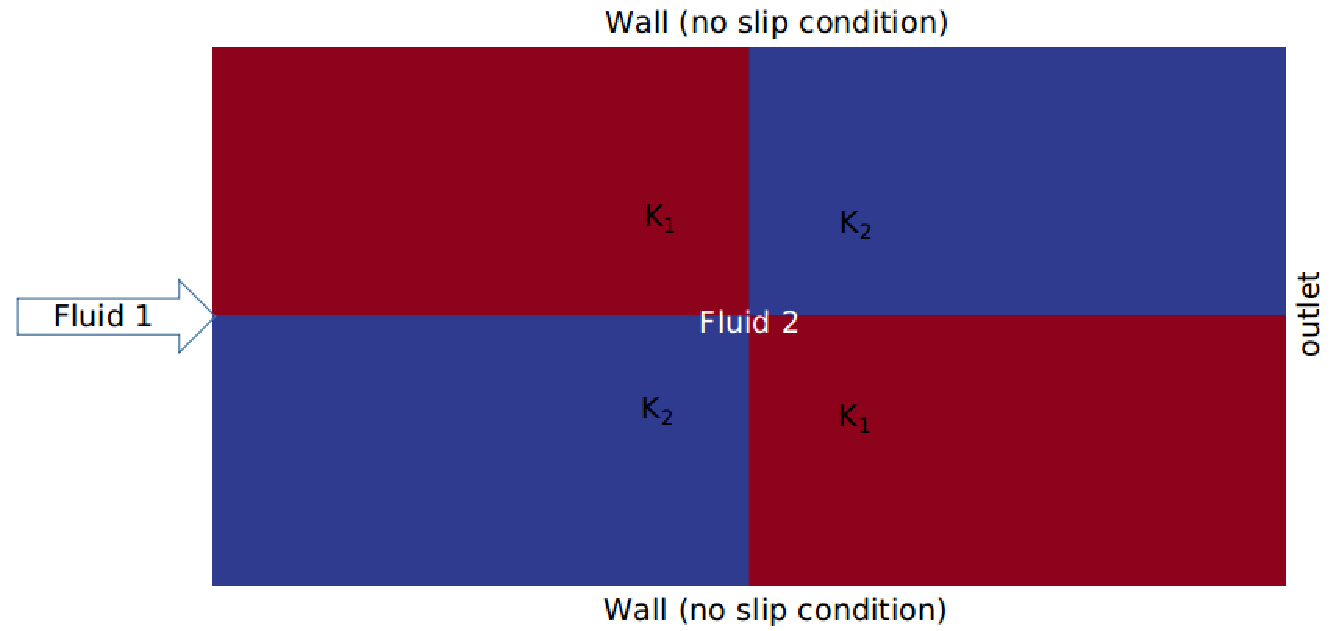
\includegraphics[width=.8\textwidth]{./Pics1/2b2_wi_fine/2b2_whole_in_fine_perm_1.pdf} 
}
\vspace{0.0cm}
\hbox{\hspace{3.5cm} (a) map of permeabilities ($\mathbf{K}$)
}
\vspace{0.25cm}
\hbox{\hspace{1.5cm}
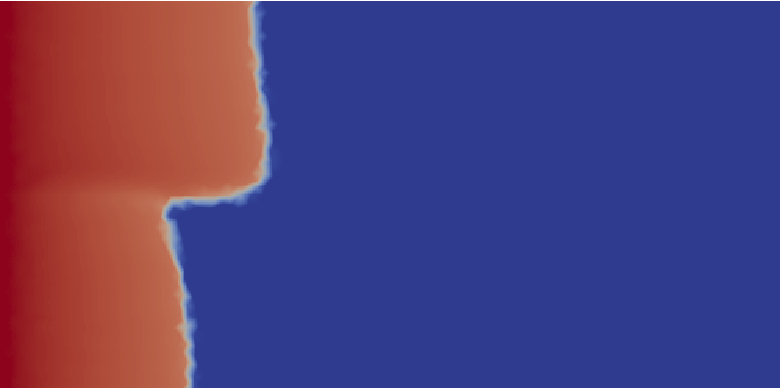
\includegraphics[width=.85\textwidth]{./Pics1/2b2_wi_fine/2b2_whole_in_fine_250_2.pdf}
}
\vspace{0.0cm}
\hbox{\hspace{4.5cm} (b) flow at t=250 
}
\vspace{0.25cm}
\hbox{\hspace{1.5cm}
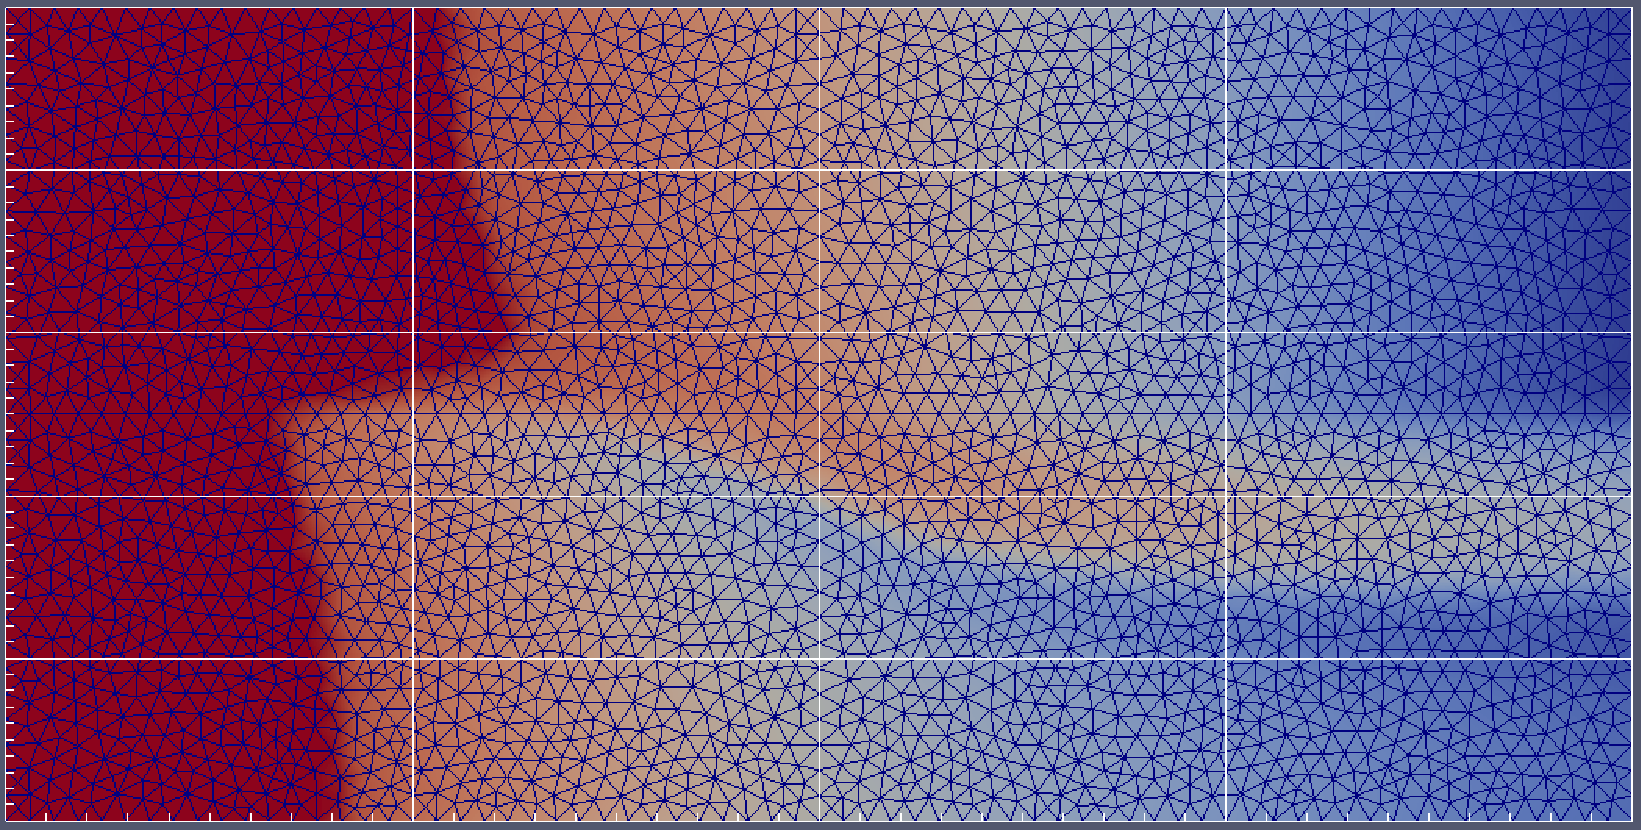
\includegraphics[width=.65\textwidth]{./Pics1/2b2_wi_fine/2b2_whole_in_fine_3000_2.pdf}
}
\vspace{0.0cm}
\hbox{\hspace{4.0cm} (c) flow at t=3000   
}}     
\caption{Model validation of fluid displacement in heterogeneous porous media ({\it VR}=1): (a) the domain is divided into four subdomains with prescribed synthetic permeability, $\mathbf{K}_{1}=1$ and $\mathbf{K}_{2}=2.5$; (b-c) snapshots of saturation (displacing fluid) field at t=$25$s and t=$300$ sec. The domain is discretised with $5960$ \PN[1]{2} elements. }
\label{fem_cv_represent_a}
\end{figure}
\clearpage



%%%%
%%%%  FIGURE
%%%%
\begin{landscape}
\begin{figure}[ht] 
\vbox{\vspace{-1cm}
\hbox{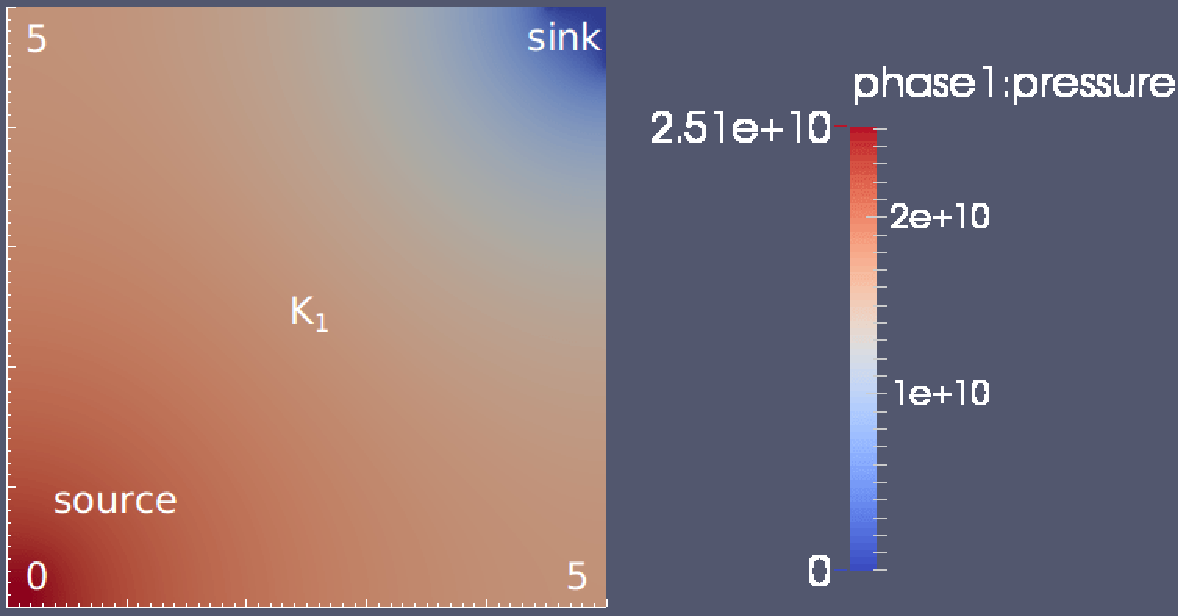
\includegraphics[width=.7\textwidth]{./Pics1/Saffman_homogeneous_MR3/saffman_homo_fixed_2.pdf}
      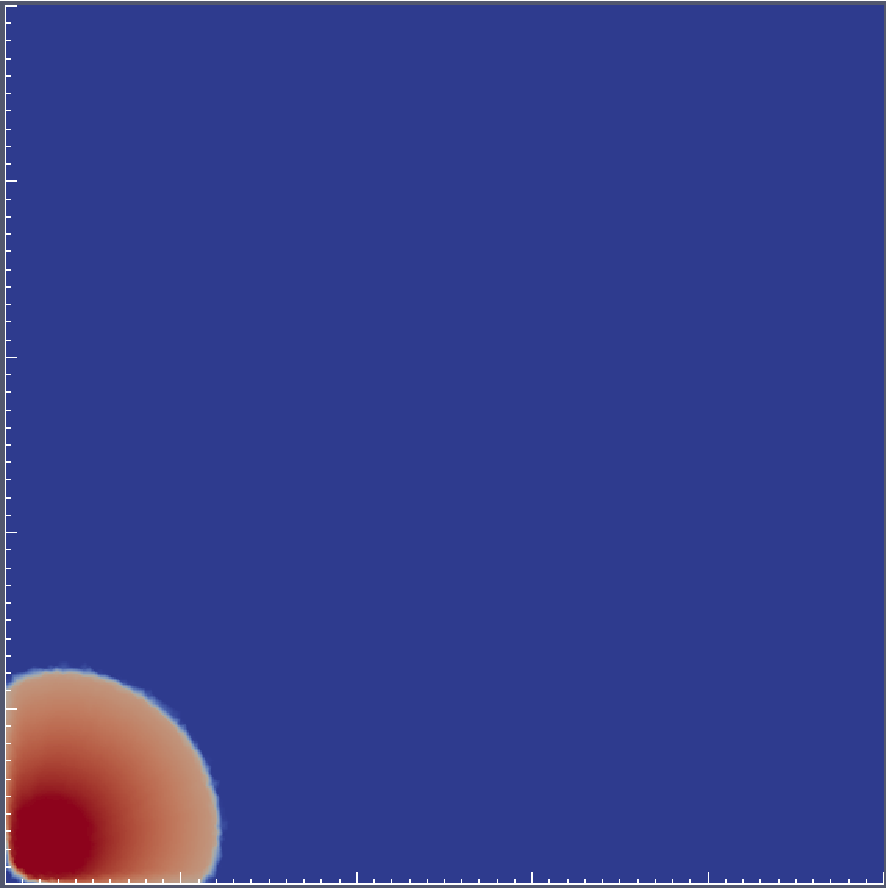
\includegraphics[width=.37\textwidth]{./Pics1/Saffman_homogeneous_MR3/saffman_homo_fixed_250.pdf}
      \includegraphics[width=.37\textwidth]{./Pics1/Saffman_homogeneous_MR3/saffman_homo_fixed_1000.pdf}}
\vspace{0.cm}
\hbox{\hspace{2.5cm} (a) pressure at t=0s \hspace{5.cm} (b) t=0.87s \hspace{2.75cm} (c) t=3.54s}
\vspace{0.5cm}
\hbox{
      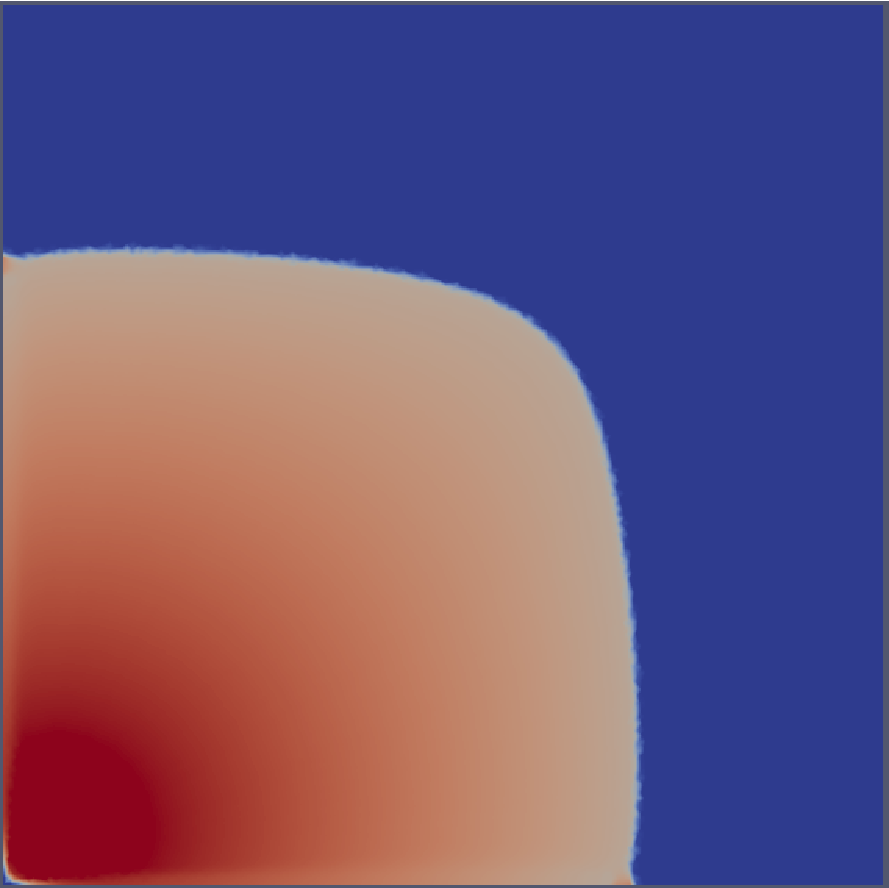
\includegraphics[width=.375\textwidth]{./Pics1/Saffman_homogeneous_MR3/saffman_homo_fixed_2500.pdf}
      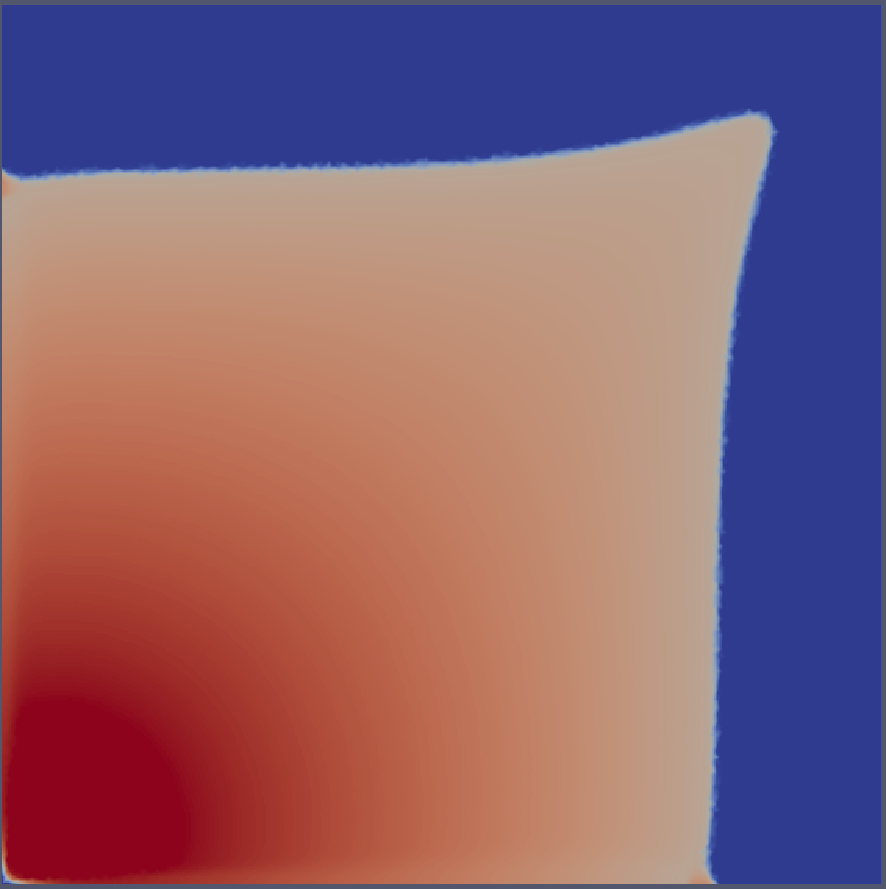
\includegraphics[width=.375\textwidth]{./Pics1/Saffman_homogeneous_MR3/saffman_homo_fixed_3500.pdf} 
      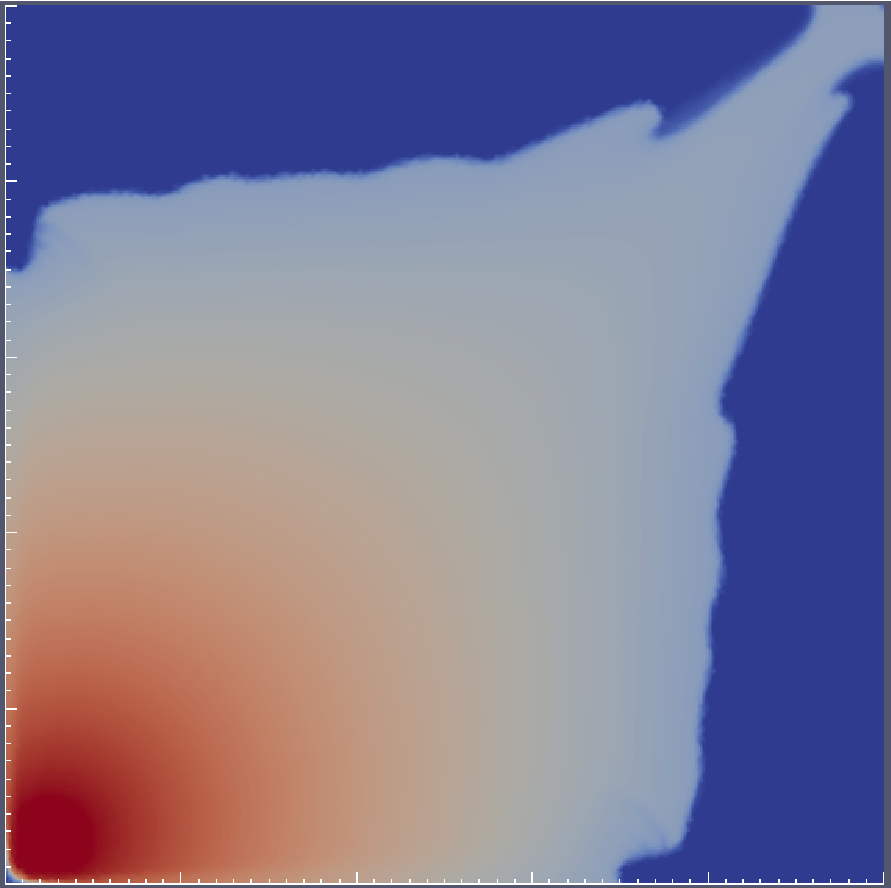
\includegraphics[width=.65\textwidth]{./Pics1/Saffman_homogeneous_MR3/saffman_homo_fixed_end.pdf}}
\vspace{0.cm}
\hbox{ \hspace{1.cm} (d) t=8.86s \hspace{3.0cm} (e) t=12.41s   \hspace{4.0cm} (f) t=17.95s}
\vspace{0.cm}
}   
\caption{Simulated flow in a Hele-Shaw cell ({\it VR}=3): (a) initial pressure profile $\left(\text{in g.cm}^{-1}\text{.s}^{-2}\right)$ with source and sink regions are explicitly shown along with dimensions (in cm); (b-f) snapshots of wetting phase saturation showing flow profile as the simulation evolves. The domain contains $47500$ \PN[1]{2} triangular elements.}
\label{fig:homoheleshaw_VN3}
\end{figure}
\end{landscape}
\clearpage



%%%%
%%%%  FIGURE
%%%%
\begin{landscape}
\begin{figure}[ht] 
\vbox{\vspace{-1cm}
\hbox{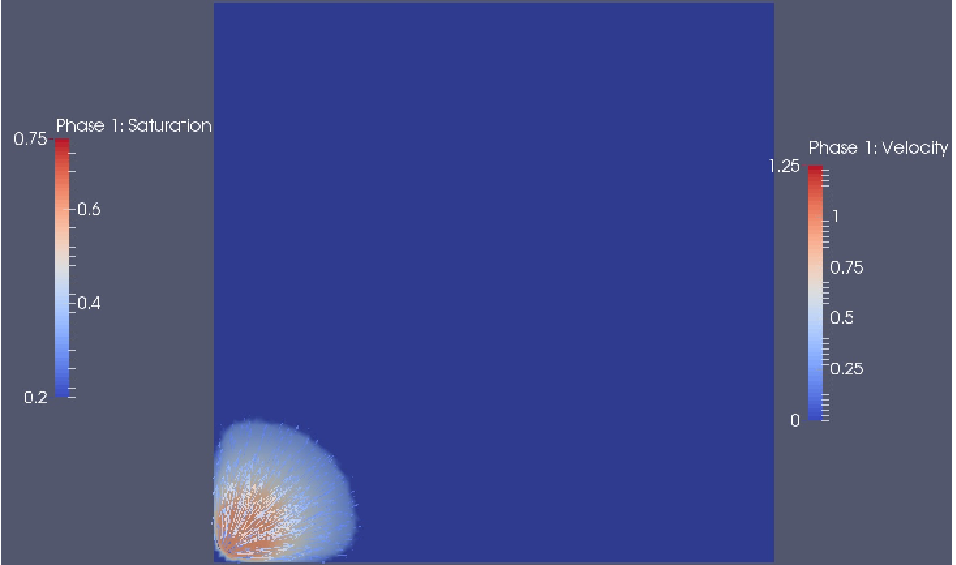
\includegraphics[width=.9\textwidth, height=0.5\textwidth]{./Pics1/Saffman_homogeneous_VR10/ST_Homog_VR10_D201c.pdf}
\hspace{0.5cm}      
      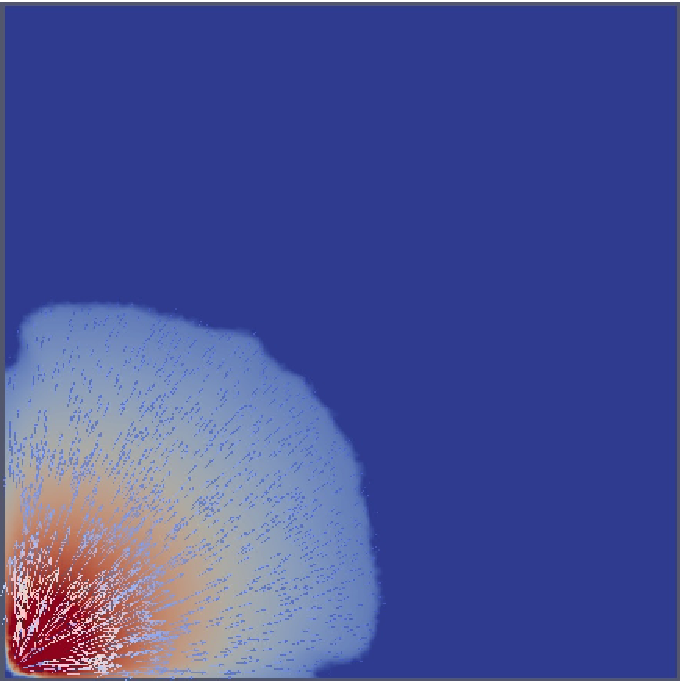
\includegraphics[width=.5\textwidth]{./Pics1/Saffman_homogeneous_VR10/ST_Homog_VR10_D1001c.pdf}}
\vspace{0.cm}
\hbox{\hspace{5.cm} (a) t=0.66s \hspace{8.cm} (b) t=3.43s }
\vspace{0.5cm}
\hbox{
      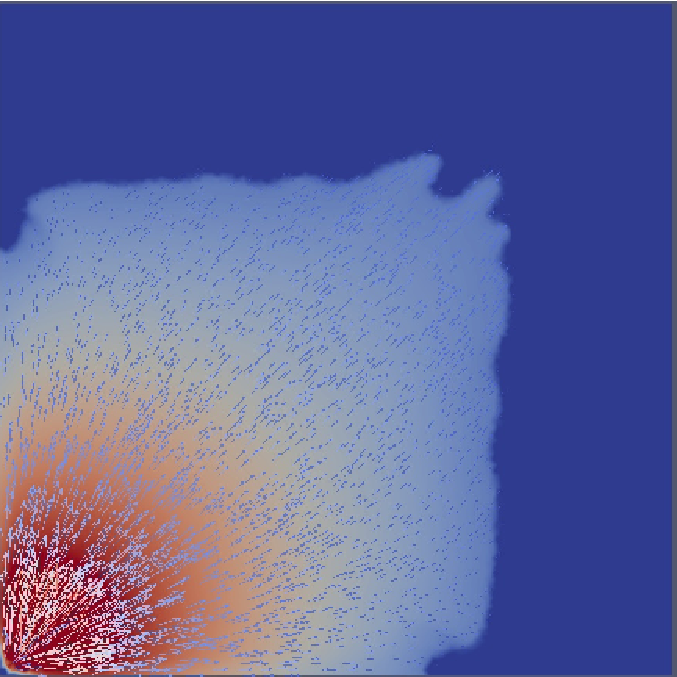
\includegraphics[width=.5\textwidth]{./Pics1/Saffman_homogeneous_VR10/ST_Homog_VR10_D2001c}
      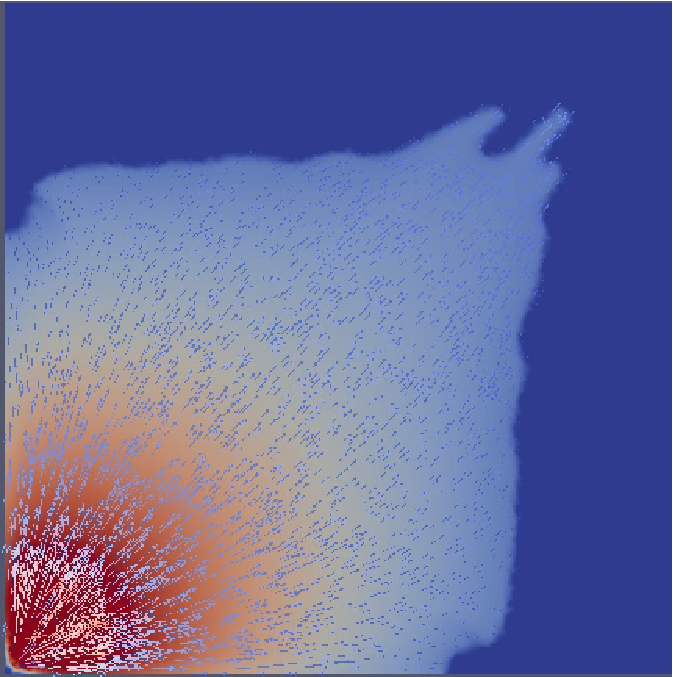
\includegraphics[width=.5\textwidth]{./Pics1/Saffman_homogeneous_VR10/ST_Homog_VR10_D2201c}
      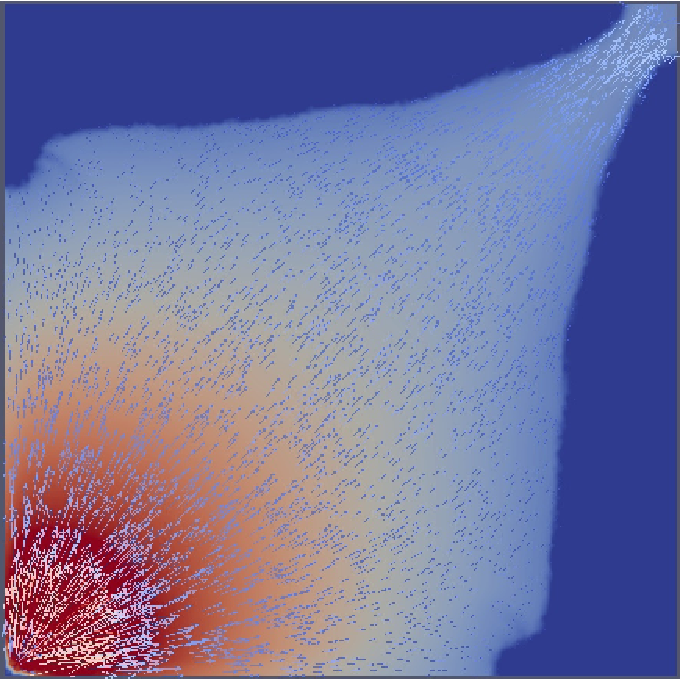
\includegraphics[width=.5\textwidth]{./Pics1/Saffman_homogeneous_VR10/ST_Homog_VR10_D3001c}}
\vspace{0.cm}
\hbox{ \hspace{2.cm} (c) t=6.92s \hspace{4.5cm} (d) t=7.61s \hspace{4.5cm} (e)t=10.00s}
\vspace{0.cm}
}   
\caption{Simulated flow in a Hele-Shaw cell ({\it VR}=10): snapshots of overlapped wetting phase saturation and velocity vectors showing flow profile as the simulation evolves. The domain contains $26313$ \PN[1]{2} triangular elements.}
\label{fig:homoheleshaw_VN10}
\end{figure}
\end{landscape}
\clearpage

%%%%
%%%%  FIGURE
%%%%
\begin{landscape}
\begin{figure}[ht] 
\vbox{\vspace{-1cm}
\hbox{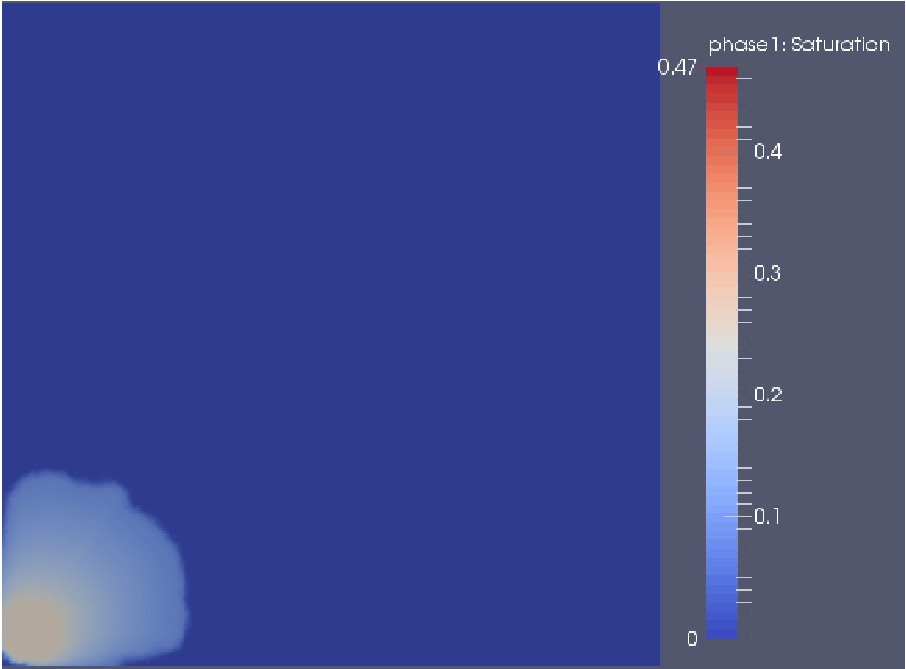
\includegraphics[width=.9\textwidth, height=0.5\textwidth]{./Pics1/Saffman_homogeneous_VR150/ST_Homog_VR150_D300b}
\hspace{0.5cm}      
      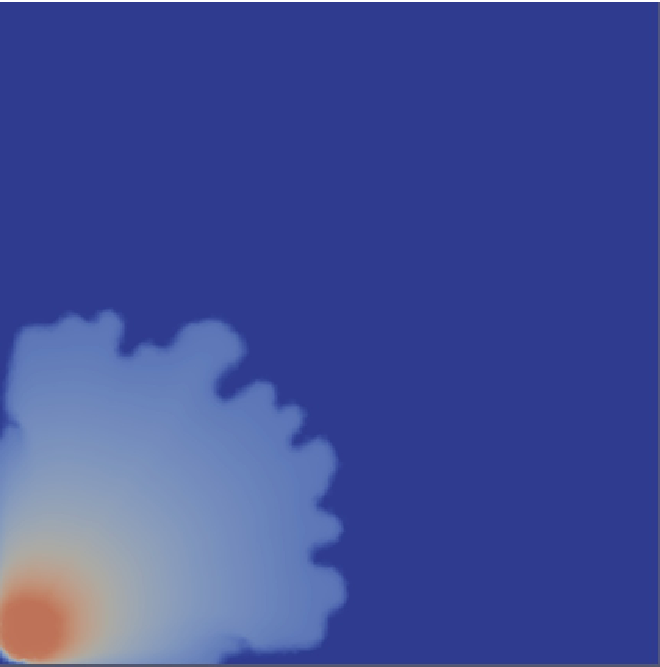
\includegraphics[width=.5\textwidth]{./Pics1/Saffman_homogeneous_VR150/ST_Homog_VR150_D1600b}}
\vspace{0.cm}
\hbox{\hspace{5.cm} (a) t=0.27s \hspace{8.cm} (b) t=0.94s }
\vspace{0.5cm}
\hbox{
      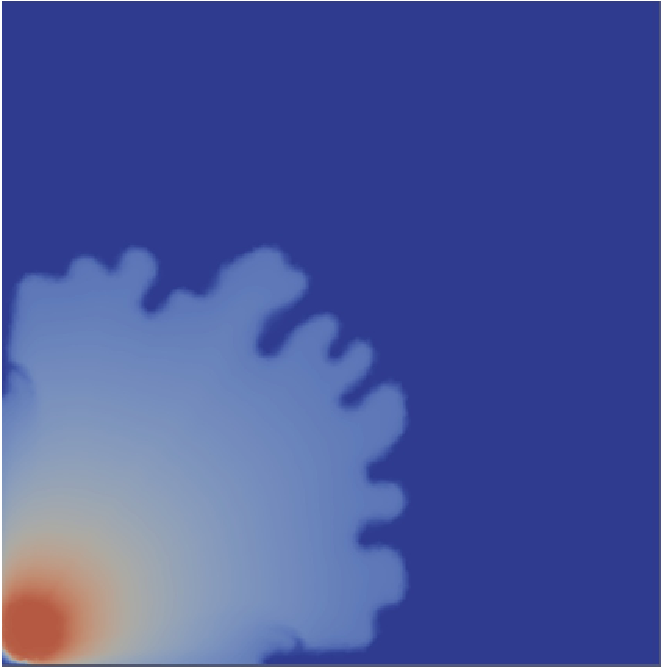
\includegraphics[width=.5\textwidth]{./Pics1/Saffman_homogeneous_VR150/ST_Homog_VR150_D2700b}
      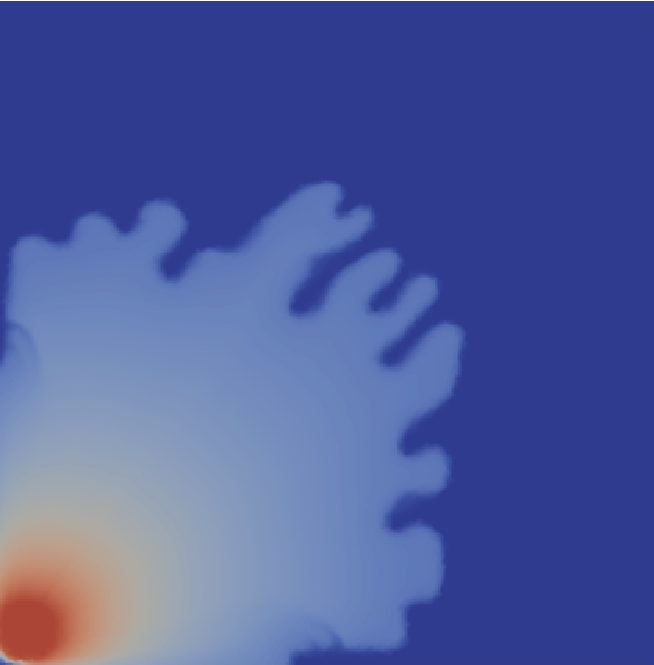
\includegraphics[width=.5\textwidth]{./Pics1/Saffman_homogeneous_VR150/ST_Homog_VR150_D4000b}
      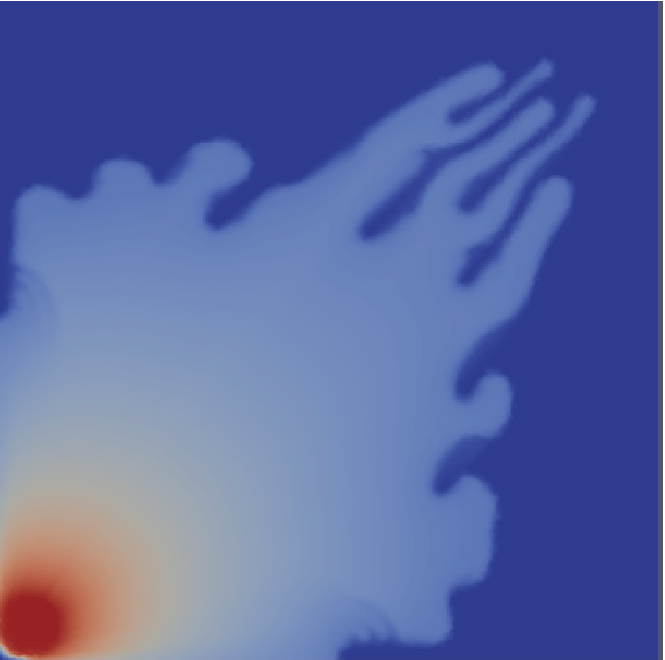
\includegraphics[width=.5\textwidth]{./Pics1/Saffman_homogeneous_VR150/ST_Homog_VR150_D7000b}}
\vspace{0.cm}
\hbox{ \hspace{2.cm} (c) t=1.32s \hspace{4.5cm} (d) t=1.70s \hspace{4.5cm} (e)t=2.31s}
\vspace{0.cm}
}   
\caption{Simulated flow in a Hele-Shaw cell ({\it VR}=150): snapshots of wetting phase saturation showing flow profile as the simulation evolves. The domain contains $26313$ \PN[1]{2} triangular elements.}
\label{fig:homoheleshaw_VN10}
\end{figure}
\end{landscape}
\clearpage


%%%%
%%%%  FIGURE
%%%%
\begin{landscape}
\begin{figure}[ht] 
\hbox{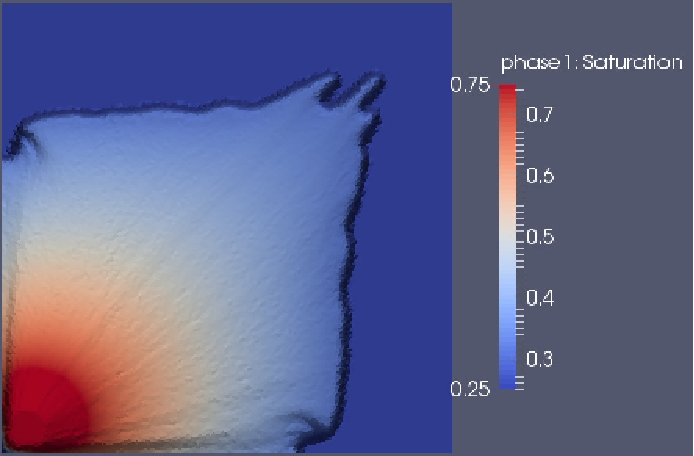
\includegraphics[width=.5\textwidth]{./Pics1/Saffman_homogeneous_VR10/ST_Homog_VR10_D2201_bbd}
       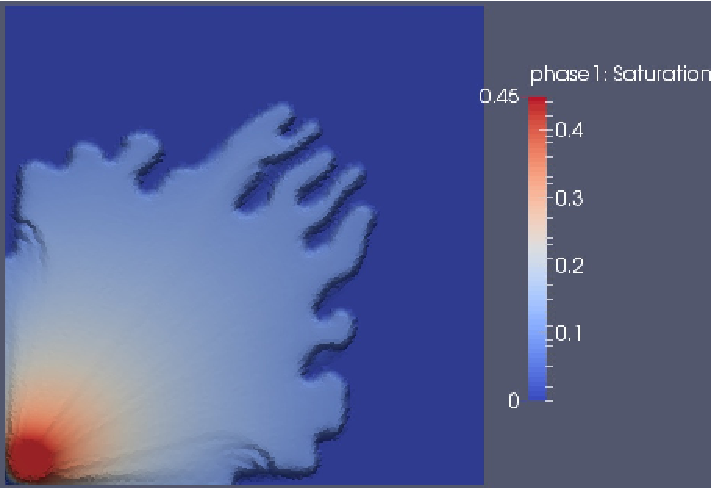
\includegraphics[width=.49\textwidth]{./Pics1/Saffman_homogeneous_VR150/ST_Homog_VR150_D5003_k2b}}
\caption{Simulated flow in Hele-Shaw cells performed with viscosity ratios of 10 (left, t=7.61s) and 150 (t=1.94s). Width of largest fingers are approximetely 0.70 and 0.90cm, which are in good agreement with values obtained from \citet{guan_2003}'s analytic solution. Domains of both simulations contain $26313$ \PN[1]{2} triangular elements.\red{(More pics to be added!!)}}
\label{fig:homoheleshaw_VN10_VN150}
\end{figure}
\end{landscape}



\begin{comment}

%%%%
%%%%  FIGURE
%%%%
\begin{landscape}
\begin{figure}[ht] 
\vbox{\vspace{-1cm}
\hbox{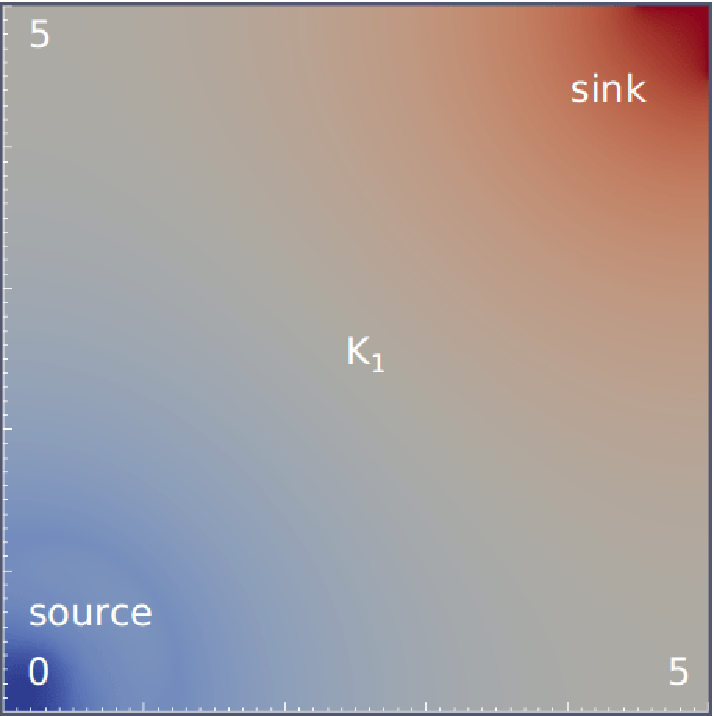
\includegraphics[width=.5\textwidth]{./Pics1/Saffman_homogeneous/saffman_homo_fixed_1.pdf}
      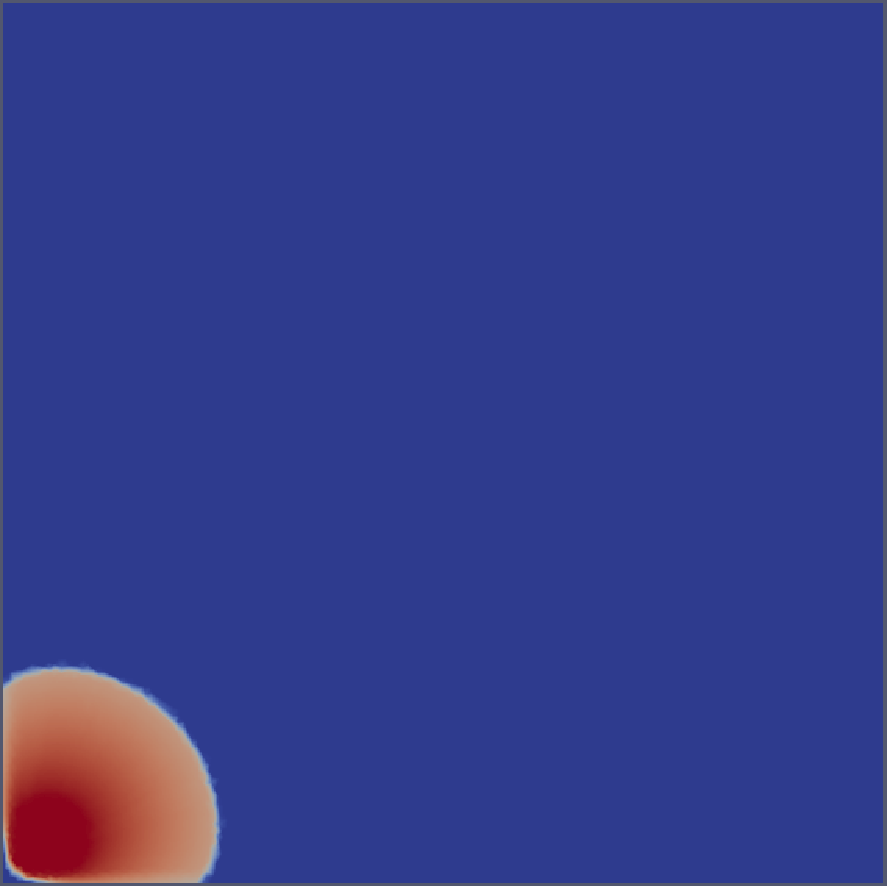
\includegraphics[width=.5\textwidth]{./Pics1/Saffman_homogeneous/saffman_homo_fixed_250_1.pdf}
      \includegraphics[width=.5\textwidth]{./Pics1/Saffman_homogeneous/saffman_homo_fixed_1000.pdf}}
\vspace{0.cm}
\hbox{\hspace{1.0cm} (a) pressure at t=0 \hspace{3.cm} (b) t=250\red{(???)} \hspace{3.0cm} (c) t=1000\red{(???)}}
\vspace{0.5cm}
\hbox{
      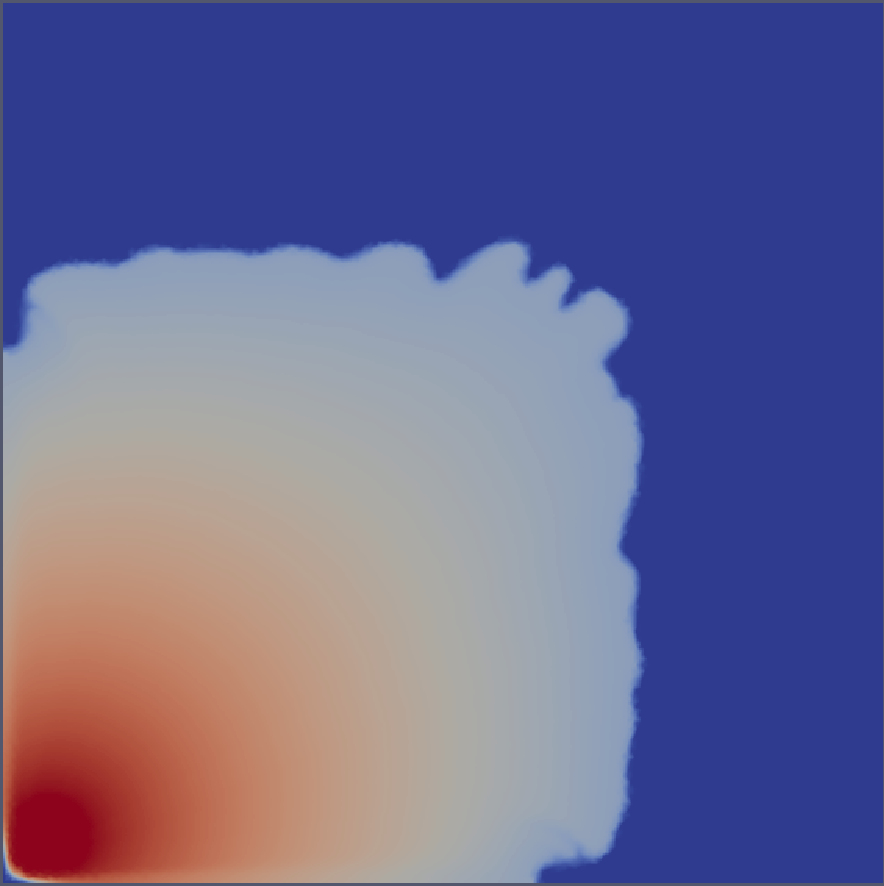
\includegraphics[width=.5\textwidth]{./Pics1/Saffman_homogeneous/saffman_homo_fixed_6000.pdf}
      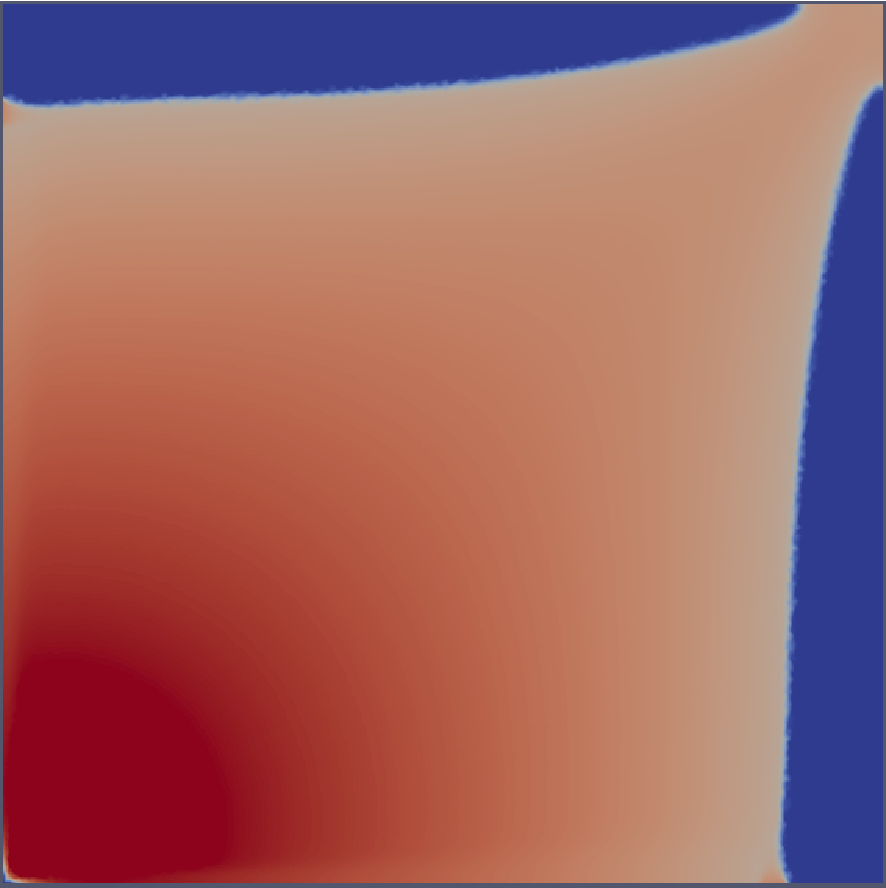
\includegraphics[width=.5\textwidth]{./Pics1/Saffman_homogeneous/saffman_homo_fixed_end_1.pdf}}
\vspace{0.cm}
\hbox{ \hspace{2.cm} (d) t=6000\red{(???)} \hspace{3.cm} (e) t=XXX\red{(???)}}
\vspace{0.cm}
}   
\caption{Simulated flow in a Hele-Shaw cell ({\it VR}=10): (a) pressure profile $\left(\text{in g.cm}^{-1}\text{.s}^{-2}\right)$ with source and sink regions explicitly shown along with dimensions (in cm); (b-e) snapshots of wetting phase saturation showing flow profile as the simulation evolves. The domain contains $47000$ \PN[1]{2} triangular elements. The pressure and saturation range of values are the same like the  case in fig.\ref{fig:homoheleshaw_VN3}.}
\label{fig:homoheleshaw_VN10}
\end{figure}
\end{landscape}
\clearpage
\end{comment}


%%%
%%% FIGURE XXXXXX
%%%
\begin{landscape}
  \begin{figure}[ht]
  \vbox{\vspace{-1cm}
      \hbox{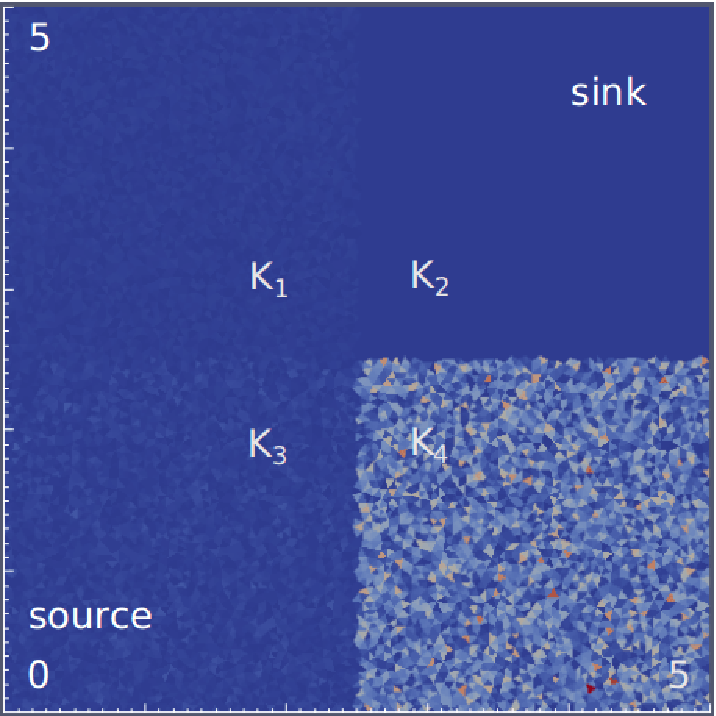
\includegraphics[width=.5\textwidth]{./Pics1/Saffman_heterogeneous/saffman_heter_fixed_1.pdf}
            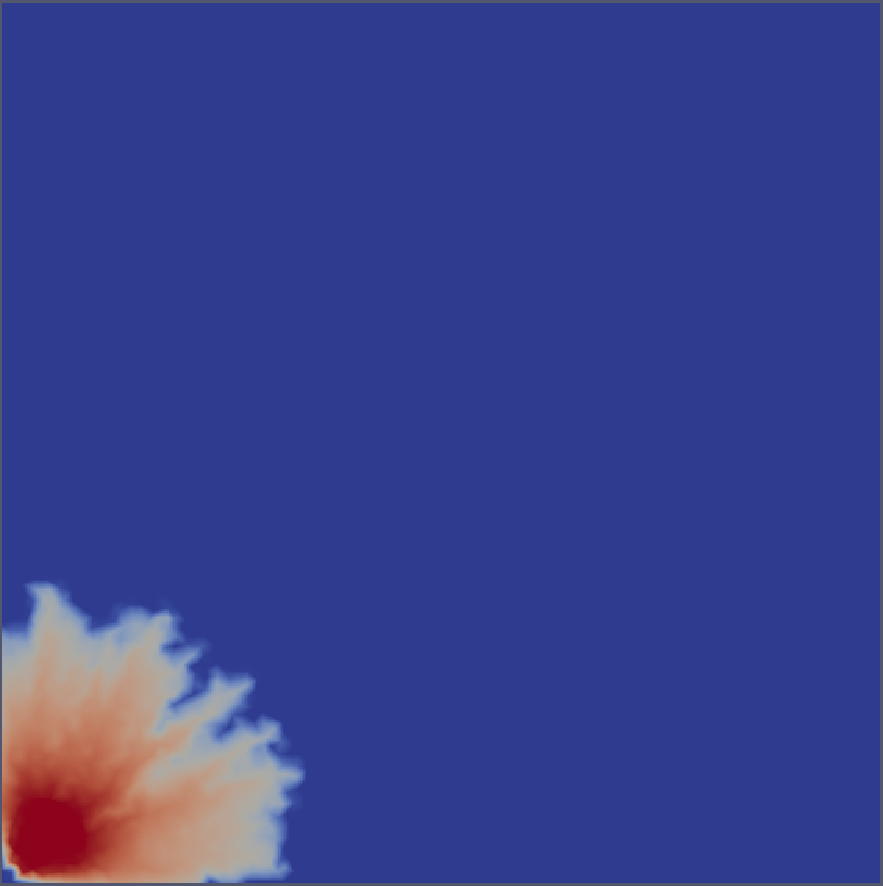
\includegraphics[width=.5\textwidth]{./Pics1/Saffman_heterogeneous/saffman_heter_fixed_500.pdf} 
            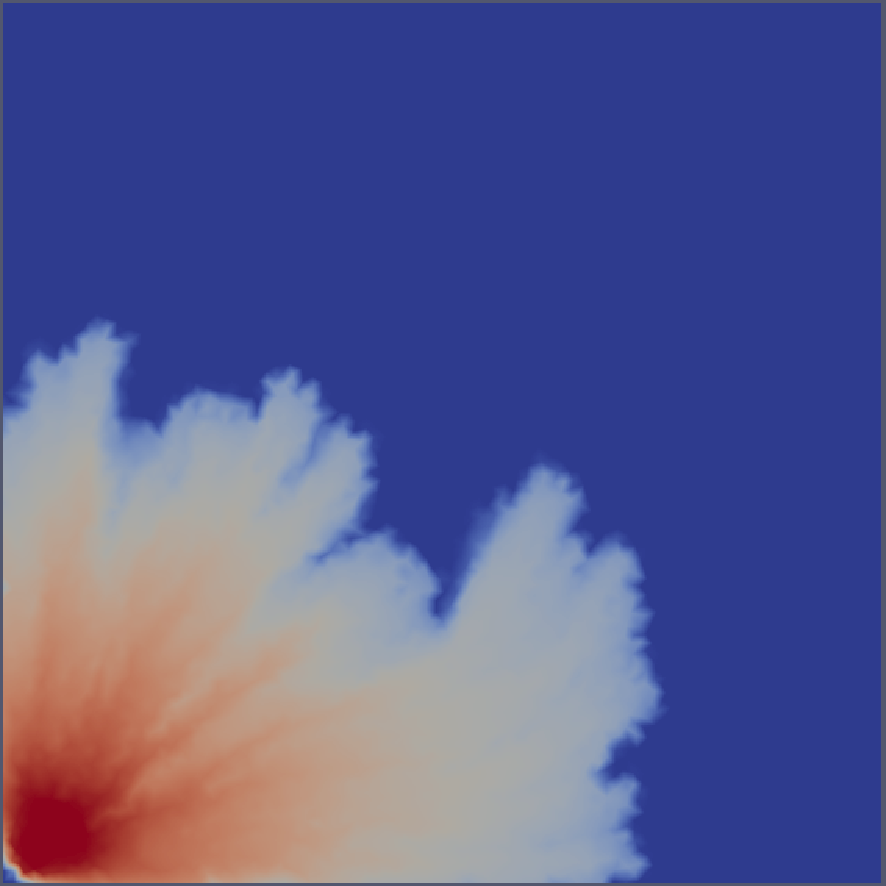
\includegraphics[width=.5\textwidth]{./Pics1/Saffman_heterogeneous/saffman_heter_fixed_2000.pdf} }
      \hbox{\hspace{1.0cm} (a) permeability map \hspace{3.cm} (b) t=0.75s \hspace{4.0cm} (c) t=8s}
      \vspace{0.5cm}
      \hbox{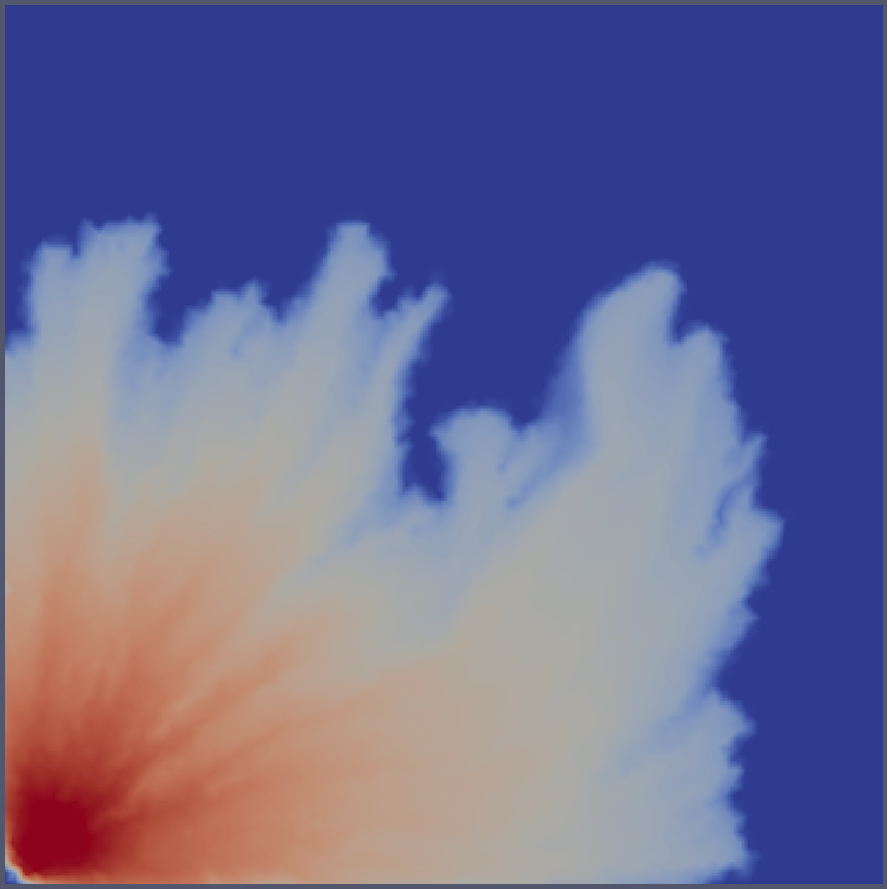
\includegraphics[width=.5\textwidth]{./Pics1/Saffman_heterogeneous/saffman_heter_fixed_3000.pdf}
            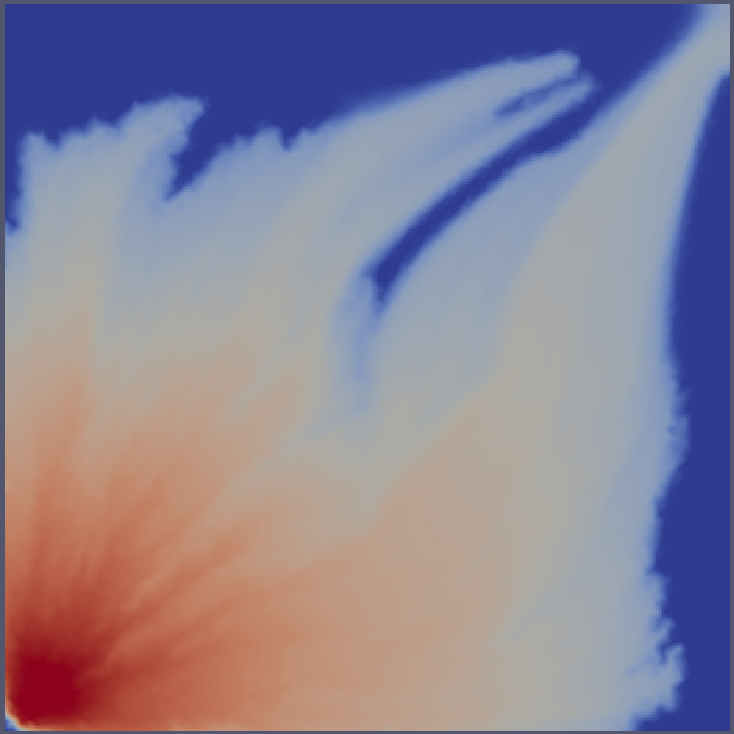
\includegraphics[width=.5\textwidth]{./Pics1/Saffman_heterogeneous/saffman_heter_fixed_6000.pdf}
            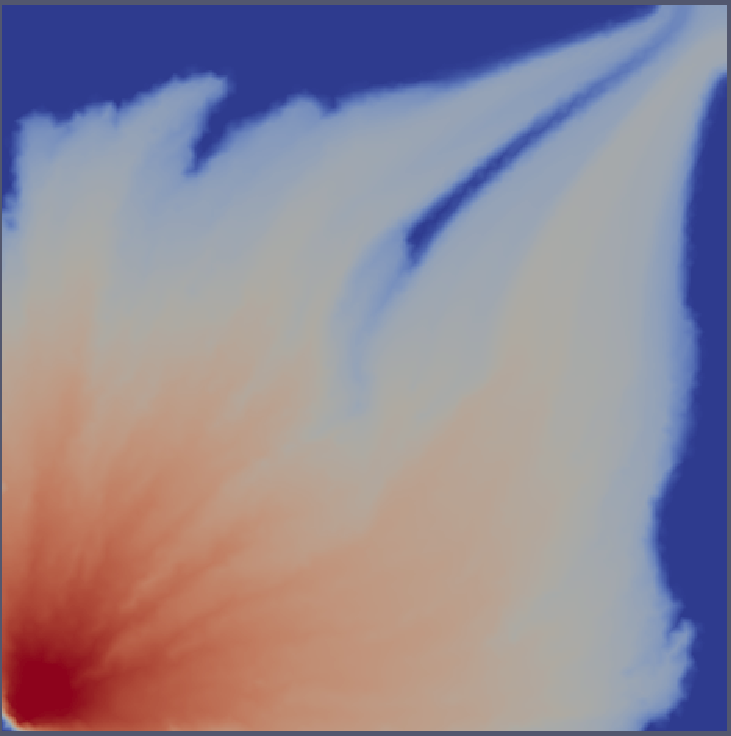
\includegraphics[width=.5\textwidth]{./Pics1/Saffman_heterogeneous/saffman_heter_fixed_24000.pdf} }
      \hbox{\hspace{2.5cm} (d) t=18s \hspace{5.cm} (e) t= \hspace{3.0cm} (f) t=24000 }}
\caption{Simulated flow in a modified Hele-Shaw cell with {\it VR}=10: (a) permeability distribution $\left(\text{10}^{-10}\le\mathbf{K}_{1}\le\text{5}\times\text{10}^{-10}\right.$, {\bf K}$_{2}$=10$^{-10}$, 10$^{-11}\le\mathbf{K}_{3}\le$ 5$\times$10$^{-10}$ and 10$^{-12}\le\mathbf{K}_{4}\le$ 5$\times$10$\left.^{-10}\text{ cm}^{2}\right)$; (b-f) snapshots of saturation profile during \red{XX} seconds of simulation. The domain contains \red{XX} \PN[1]{2} element-pairs.}
\label{fig:HeleShawHeter_VR10}
\end{figure}
\end{landscape}
\clearpage



%%%%
%%%%  FIGURE
%%%%
\begin{landscape}
\begin{figure}[ht] 
\vbox{
\hbox{\hspace{4.0cm}
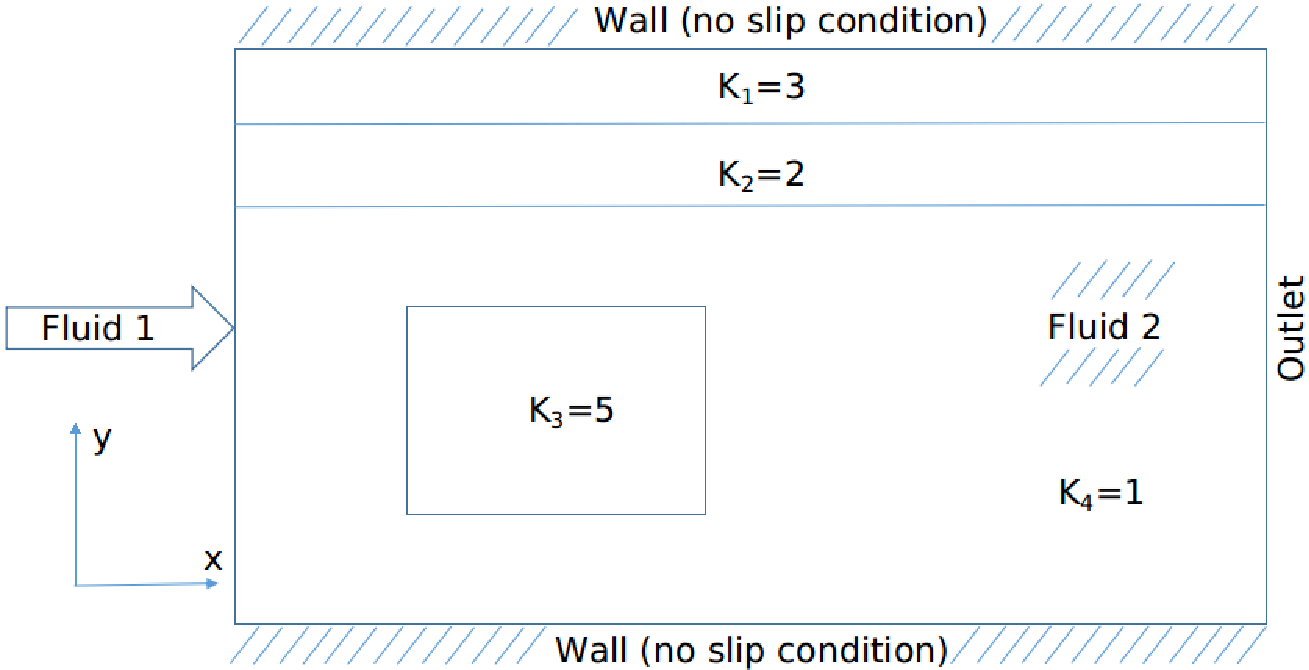
\includegraphics[width=.75\textwidth]{./Pics/map_of_boundaries.pdf} 
}
\vspace{0.0cm}
\hbox{\hspace{6.5cm} (a) map of permeabilties K   
}
\vspace{0.25cm}
\hbox{\hspace{4.0cm}
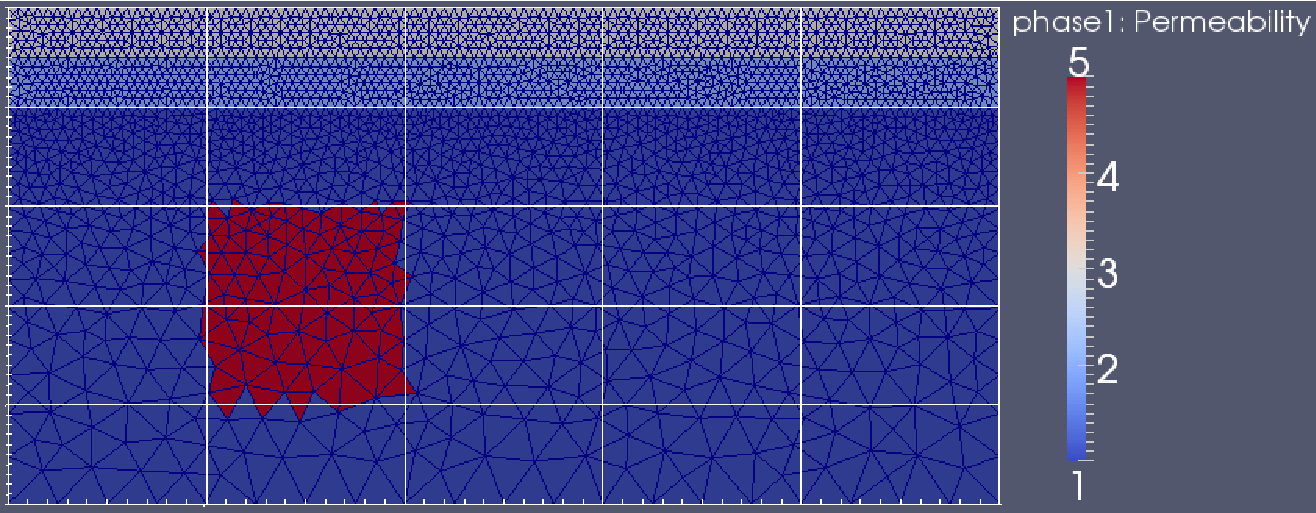
\includegraphics[width=.9\textwidth]{./Pics/map_of_boundaries_1.pdf}
}
\vspace{0.0cm}
\hbox{\hspace{9cm} (b)      
}
}     
\caption{Figure (a) describes the initial and boundary conditions as these are applied in this set of simulations. Below (b) there is a comparison between the unstructured and fixed mesh and the unstructured and adaptive mesh. During the implementation of fixed mesh initially there $4606$ elements while for the adaptive mesh there are $606$ while the majority of them is on the interface between between the two fluids. }
\label{fig:testcase_heter_domain}
\end{figure}
\end{landscape}
\clearpage



%%%%
%%%%  FIGURE
%%%%
\begin{landscape}
\begin{figure}[ht] 
\vbox{
\hbox{\hspace{3.5cm}
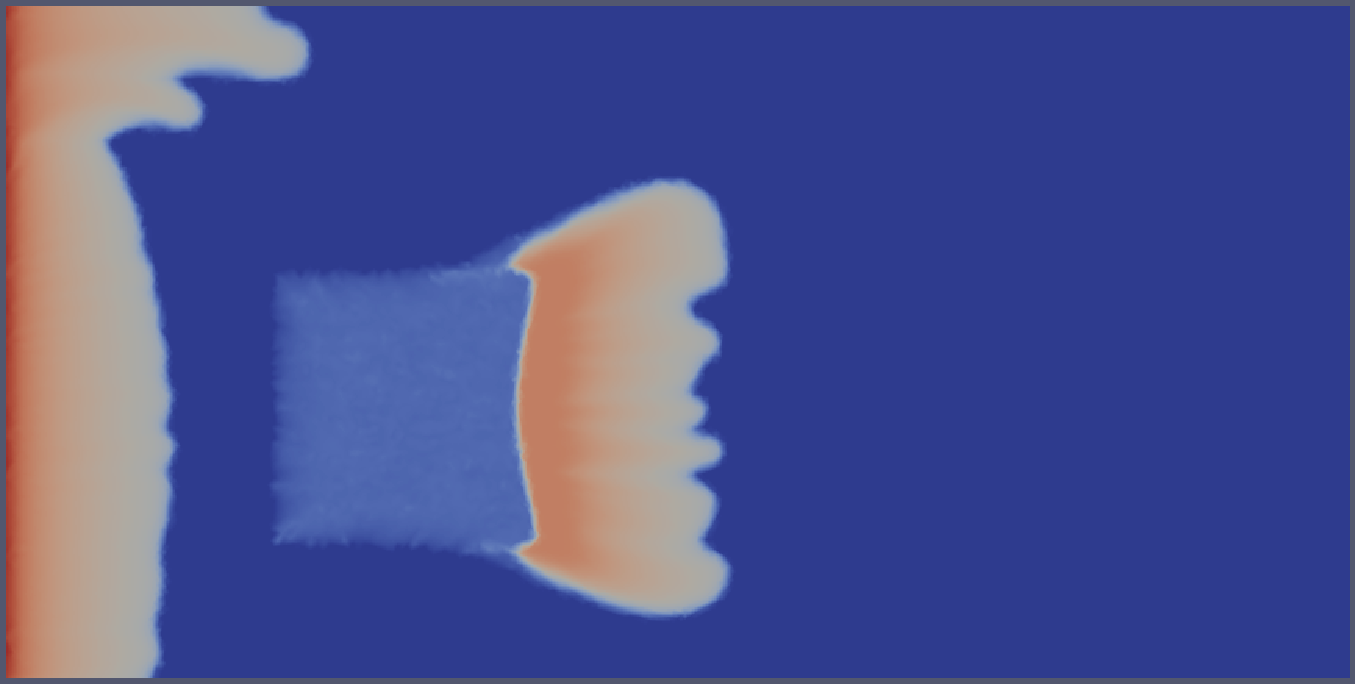
\includegraphics[width=.65\textwidth]{./Pics1/mr10_5regions_fixed/5regions_fixed_250.pdf} 
}
\vspace{0.0cm}
\hbox{\hspace{6.5cm} (a) flow at t=250 (fixed mesh)  
}
\vspace{0.25cm}
\hbox{\hspace{3.5cm}
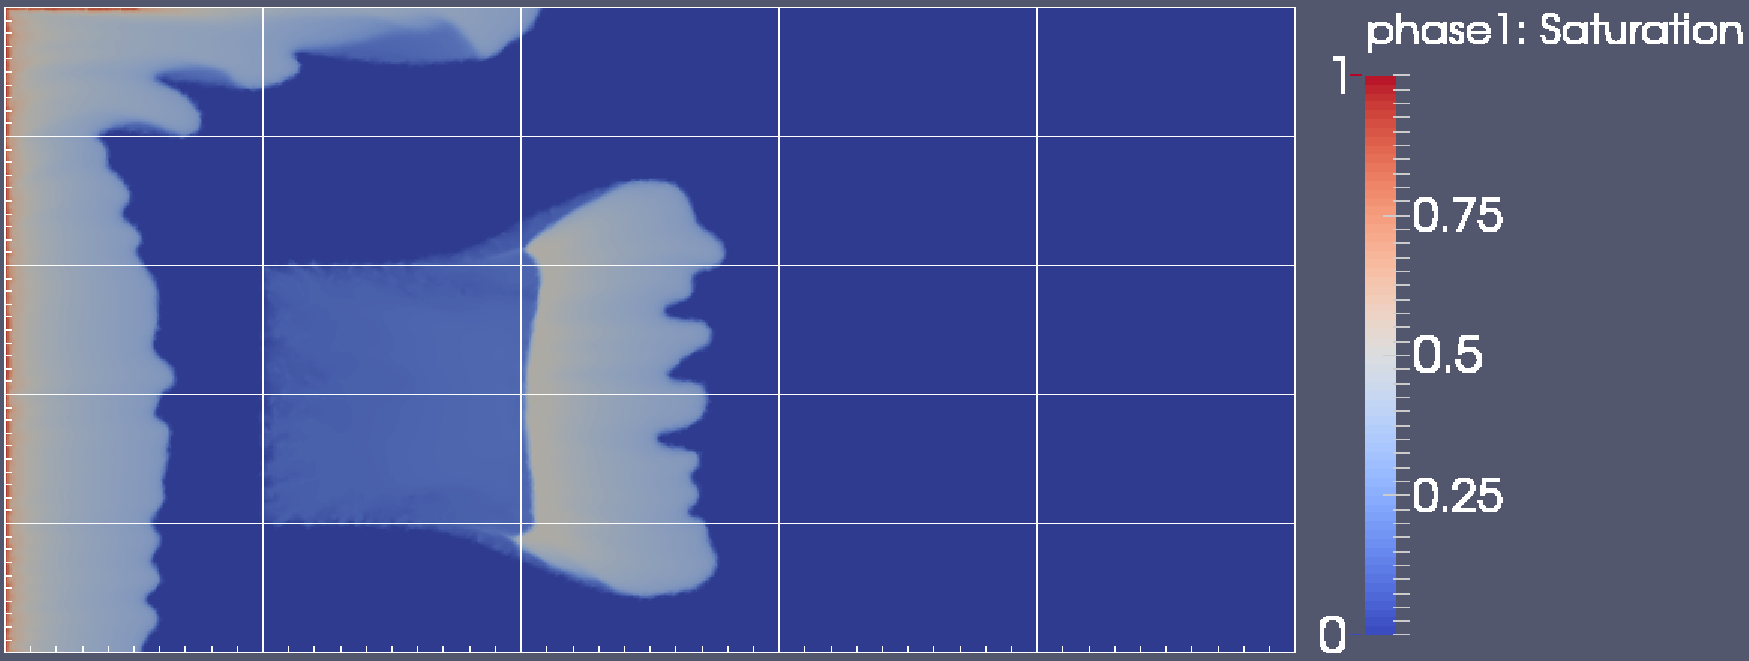
\includegraphics[width=.9\textwidth]{./Pics1/mr10_5regions_adapt/5regions_adapt_250_1.pdf}
}
\vspace{0.0cm}
\hbox{\hspace{6.5cm} (b) flow at t=250 (adaptive mesh)    
}
}     
\caption{For $t=0.125$s, $2$ test-cases under the VR=$10$ and under fixed (top) and adaptive(bottom) mesh are compared. There is a significant difference on the main front (left hand side of the domain) and the number of finger that appear.}
\label{fig:2testcase_a}
\end{figure}
\end{landscape}
\clearpage


%%%%
%%%%  FIGURE
%%%%
\begin{landscape}
\begin{figure}[ht] 
\vbox{
\hbox{\hspace{3.5cm}
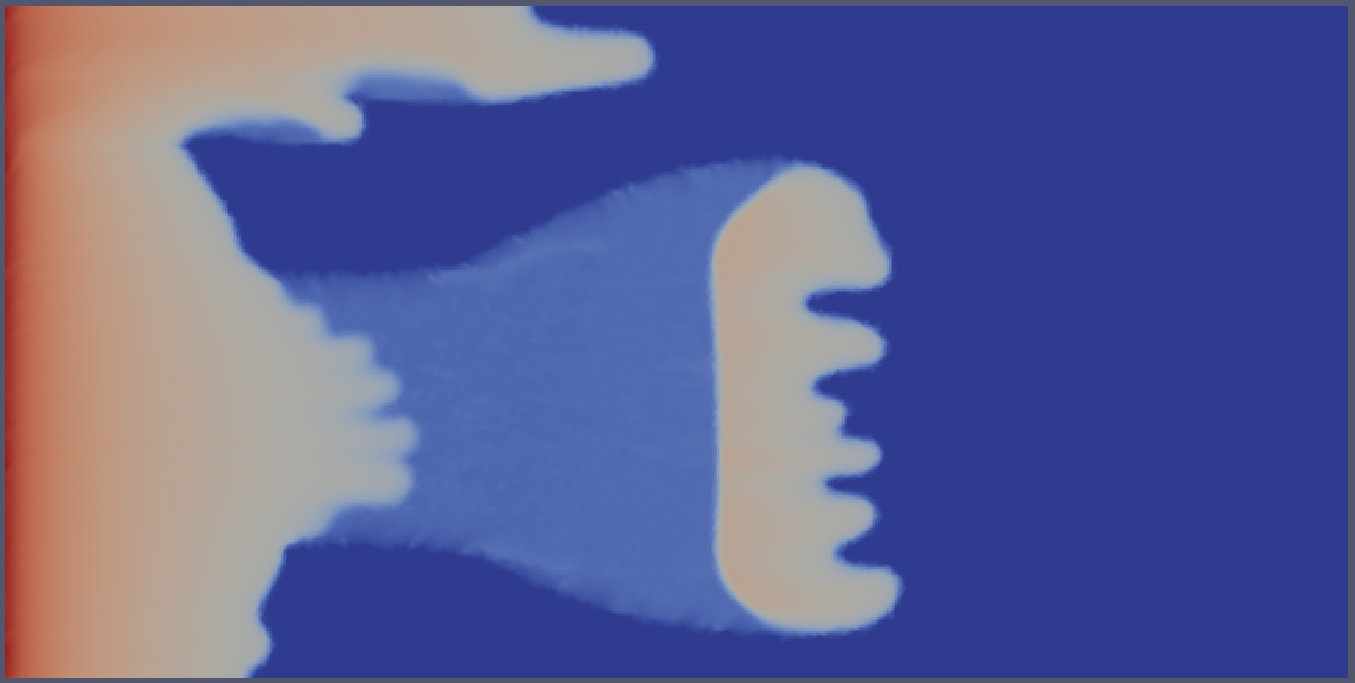
\includegraphics[width=.65\textwidth]{./Pics1/mr10_5regions_fixed/5regions_fixed_500.pdf} 
}
\vspace{0.0cm}
\hbox{\hspace{6.5cm} (a) flow at t=500 (fixed mesh)   
}
\vspace{0.25cm}
\hbox{\hspace{3.5cm}
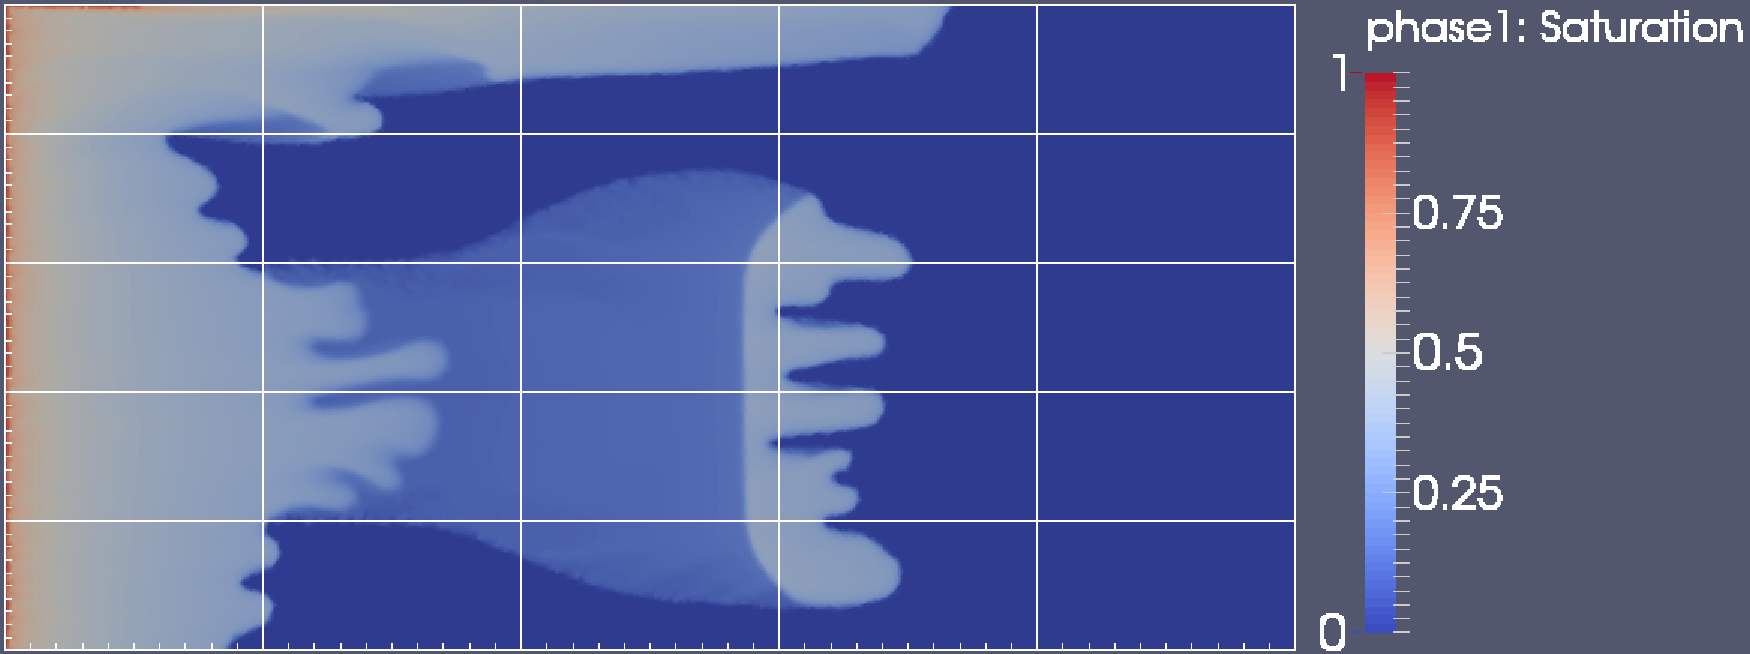
\includegraphics[width=.9\textwidth]{./Pics1/mr10_5regions_adapt/5regions_adapt_500_1.pdf}
}
\vspace{0.0cm}
\hbox{\hspace{6.5cm} (b) flow at t=500 (adaptive mesh)     
}
}     
\caption{At $t=0.25$s ($t=500$, timestemp) cross flow is taking place at the upper part of the formation. The fingers start to becoming more proufound as can been seen at the bottom.}
\label{fig:2testcase_b}
\end{figure}
\end{landscape}
\clearpage



%%%%
%%%%  FIGURE
%%%%
\begin{landscape}
\begin{figure}[ht] 
\vbox{
\hbox{\hspace{3.5cm}
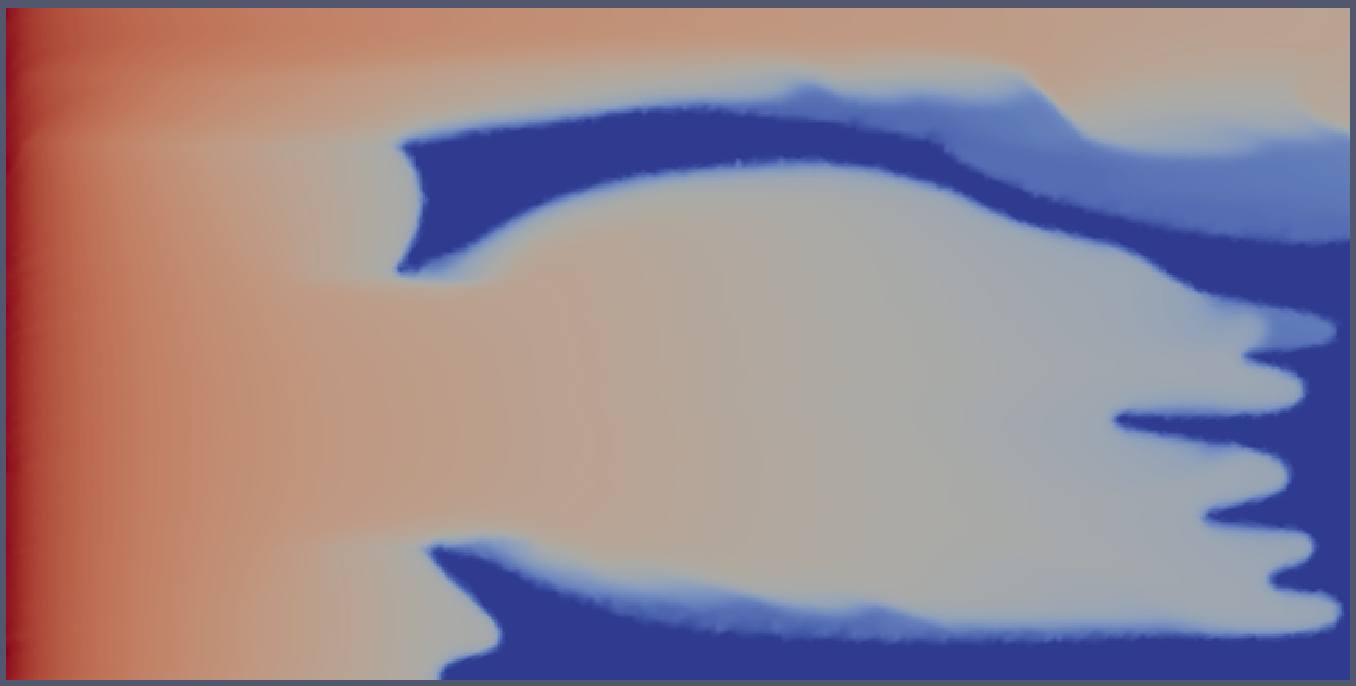
\includegraphics[width=.65\textwidth]{./Pics1/mr10_5regions_fixed/5regions_fixed_1500.pdf} 
}
\vspace{0.0cm}
\hbox{\hspace{6.5cm} (a) flow at t=1500 (fixed mesh)   
}
\vspace{0.25cm}
\hbox{\hspace{3.5cm}
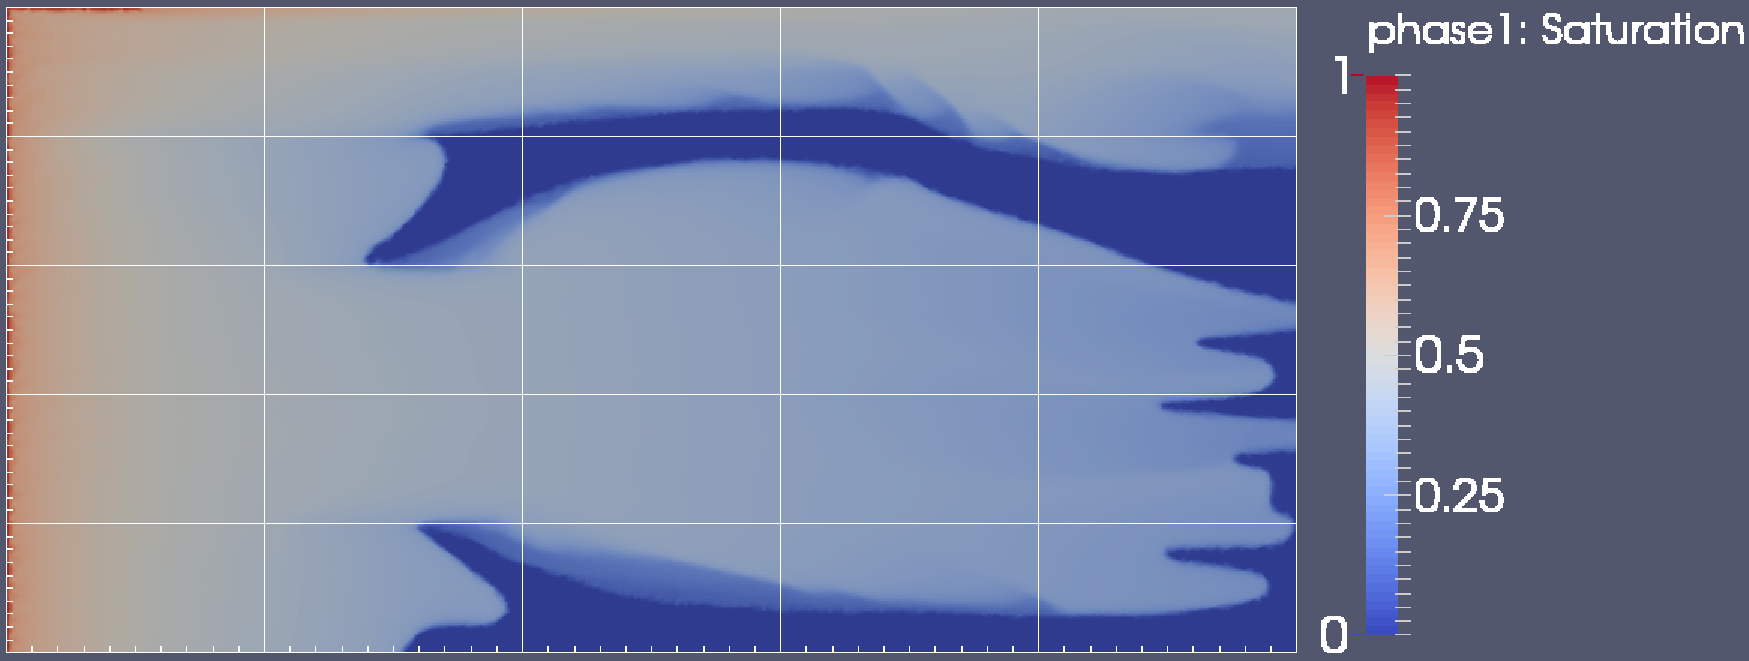
\includegraphics[width=.9\textwidth]{./Pics1/mr10_5regions_adapt/5regions_adapt_1500_1.pdf}
}
\vspace{0.0cm}
\hbox{\hspace{6.5cm} (b) flow at t=1500 (adaptive mesh)     
}
}     
\caption{At $t=0.75 sec$ ($t=1500$, timestemp) the initial cross flow is now fully developed and has travel all the way towards the outlet (right-hand side). and the finger below start forming a front that is also travelling towards the left-hand side.}
\label{fig:2testcase_c}
\end{figure}
\end{landscape}
\clearpage



%%%%
%%%%  FIGURE
%%%%
\begin{landscape}
\begin{figure}[ht] 
\vbox{
\hbox{\hspace{3.5cm}
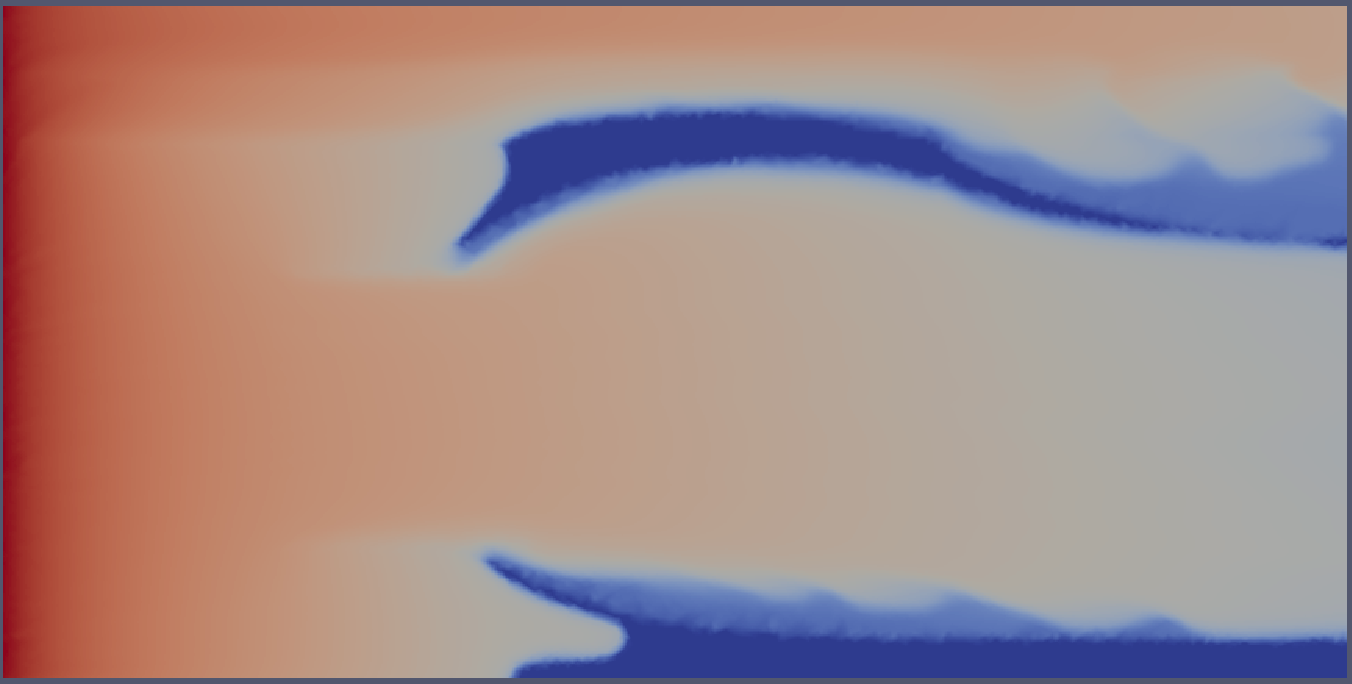
\includegraphics[width=.65\textwidth]{./Pics1/mr10_5regions_fixed/5regions_fixed_2000.pdf} 
}
\vspace{0.0cm}
\hbox{\hspace{6.5cm} (a) flow at t=end (fixed mesh)   
}
\vspace{0.25cm}
\hbox{\hspace{3.5cm}
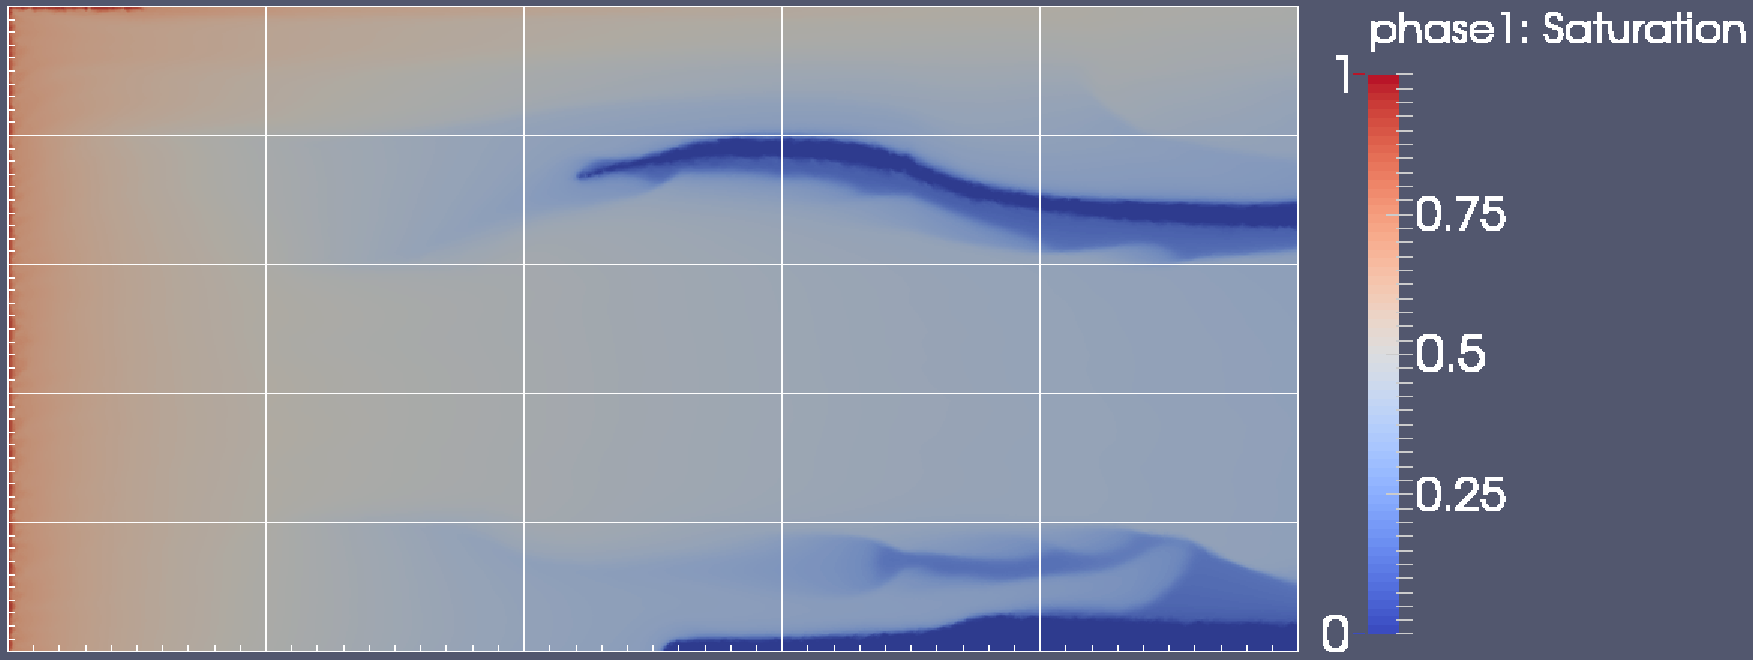
\includegraphics[width=.9\textwidth]{./Pics1/mr10_5regions_adapt/5regions_adapt_3000_1.pdf}
}
\vspace{0.0cm}
\hbox{\hspace{6.5cm} (b) flow at t=end (adaptive mesh)     
}
}     
\caption{Using the $P_{1}DGP_{2}$ element type for VR=$10$ under the same time steps, we compared the impact of fixed and adaptive mesh for the same timeframe. The end of simulation happens at $time=5 sec$ and for the timestemp $t=9999$ while the number of elements in both simulations was approximately $4700$. When adaptive mesh is introduce there is better repersentation of the fluid instabilities as these are developed on time.}
\label{fig:2testcase_d}
\end{figure}
\end{landscape}
\clearpage



%%%%
%%%%  FIGURE
%%%%
\begin{landscape}
\begin{figure}[ht] 
\vbox{
\hbox{\hspace{3.5cm}
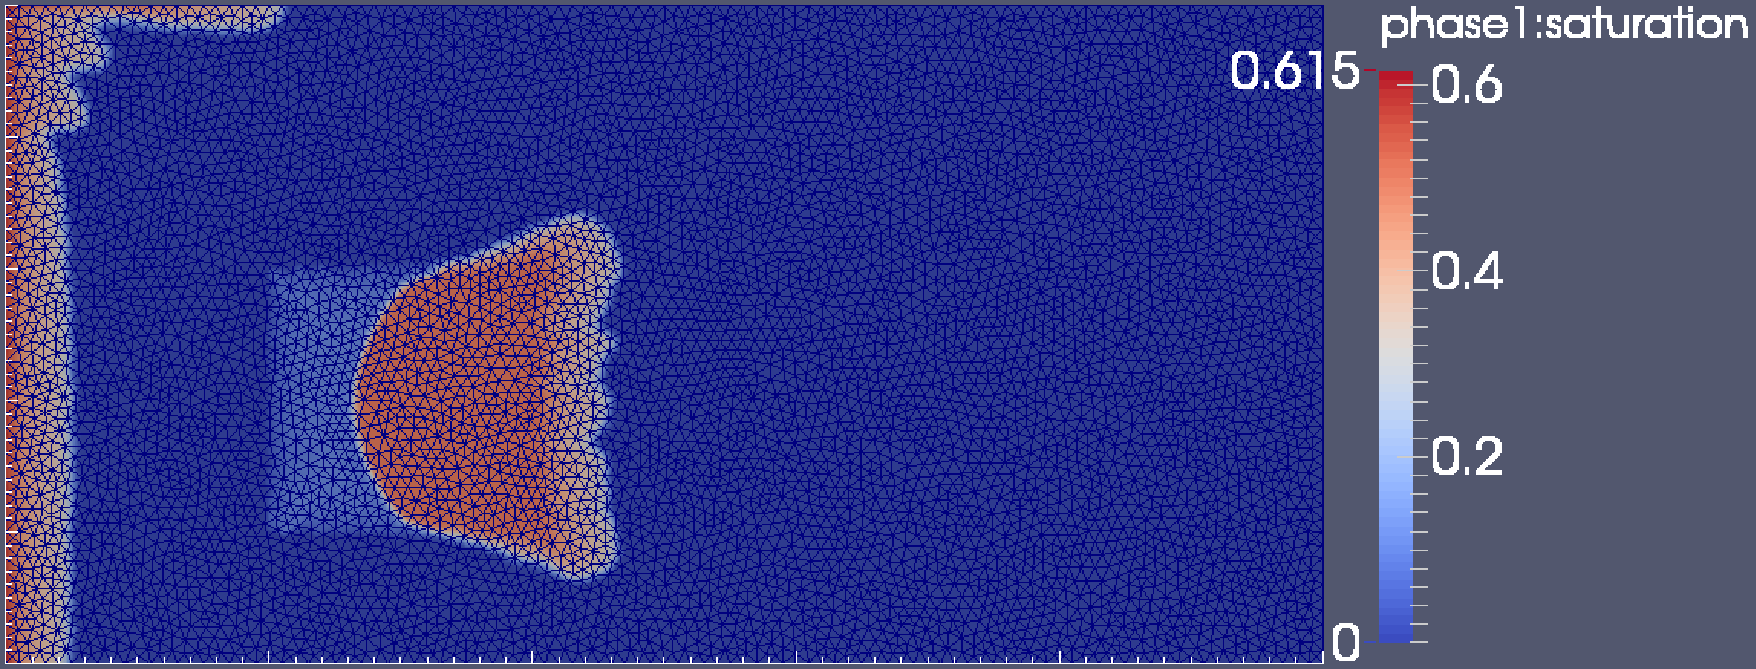
\includegraphics[width=.9\textwidth]{./Pics1/mr10_5regions_fixed_dinlet/5regions_dinlet_fixed_100_1.pdf}
}
\vspace{0.0cm}
\hbox{\hspace{6.5cm} (a) double inlet - fixed mesh   
}
\hbox{\hspace{3.5cm}
  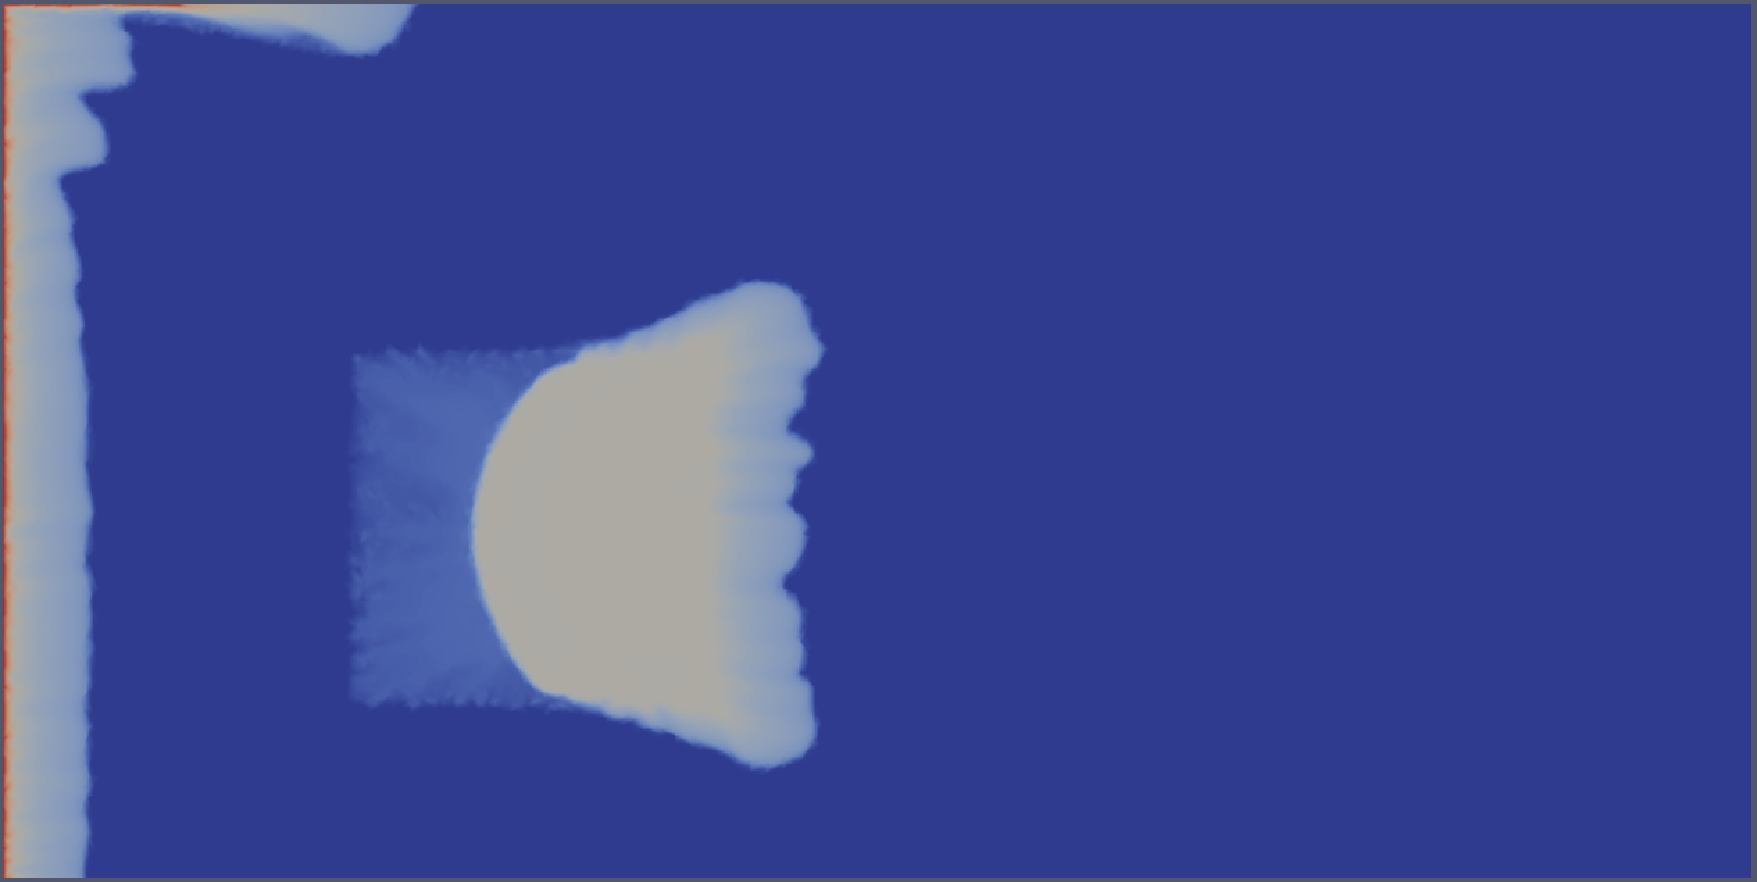
\includegraphics[width=.67\textwidth]{./Pics1/mr10_5regions_adapt_dinlet/5regions_dinlet_adapt_start.pdf}
}
\vspace{0.0cm}
\hbox{\hspace{6.5cm} (b) double inlet adaptive mesh   
}
}     
\caption{Comparing test-cases of fixed and adaptive mesh while a second region/inlet is introduced. For $t=0.101$s, using the $P_{1}DGP_{2}$ element type for MR=$10$ under the same time steps. For this simulation there are $13226$ elements for the fixed messh and $43716$ for the adaptive.}
\label{fig:3testcase_a}
\end{figure}
\end{landscape}
\clearpage

%%%%
%%%%  FIGURE
%%%%
\begin{figure}[ht] 
\vbox{
\hbox{\hspace{3.5cm}
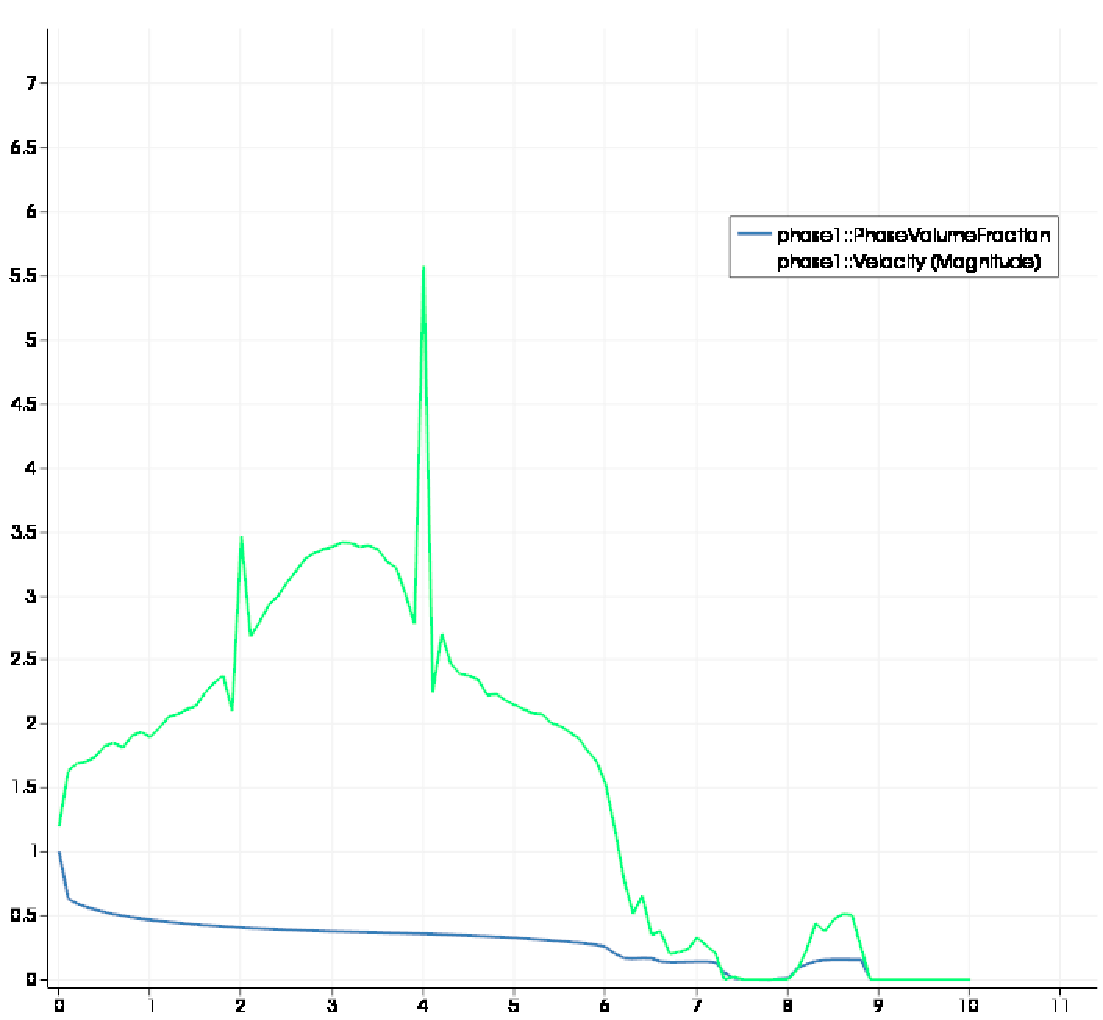
\includegraphics[width=.5\textwidth]{./Pics1/mr10_5regions_adapt/5regions_adapt_vel_magn.pdf} 
}
\vspace{0.0cm}
\hbox{\hspace{5.0cm} (a) single inlet velocity magnitude   
}
\hbox{\hspace{3.5cm}
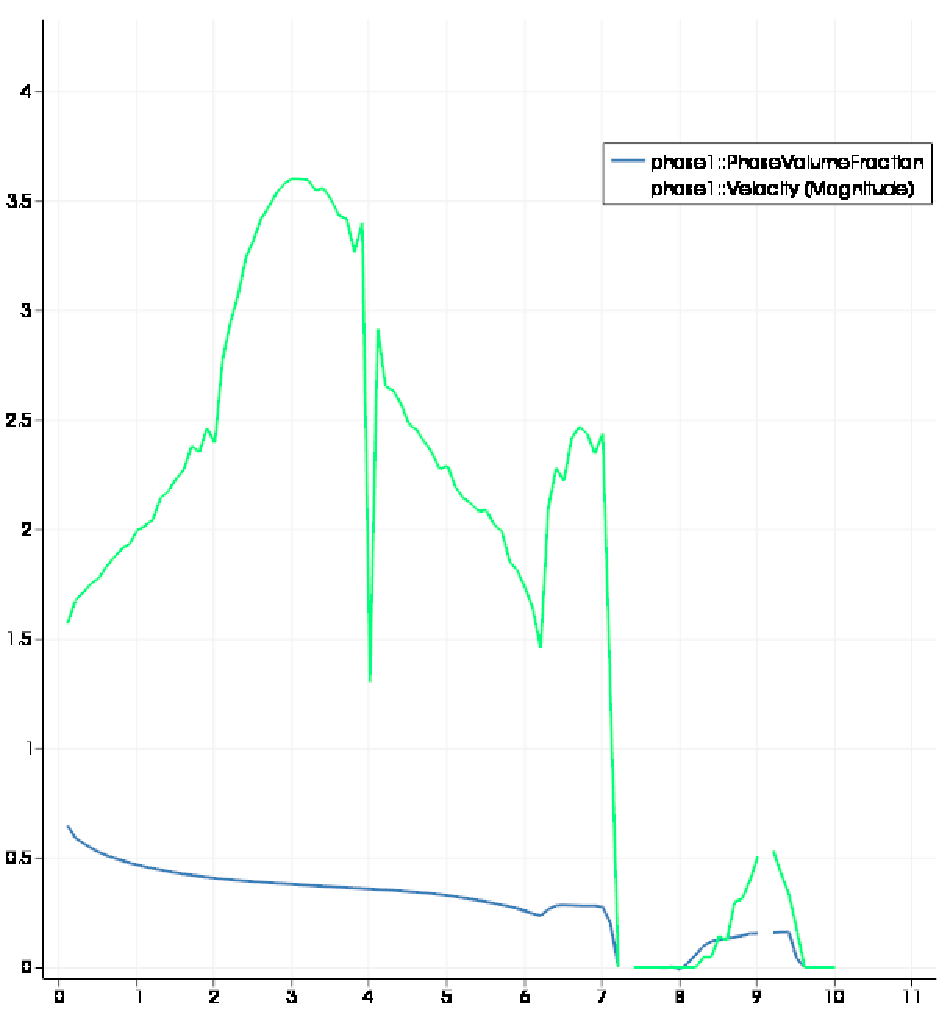
\includegraphics[width=.5\textwidth]{./Pics1/mr10_5regions_adapt_dinlet/5regions_dinlet_adapt_vel_magn.pdf}
}
\vspace{0.0cm}
\hbox{\hspace{5.0cm} (b) double inlet velocity magnitude   
}
}     
\caption{For the same time step, t=1000, these plots describe the velocity magnitudes of the phase $1$ (injected fluid) under the same boundary and initiall conditions. From top to bottom,these graphs describe the velocity magnitude %for fixed mesh is plotted(top), the velocity magnitude 
for adaptive mesh-single inlet (top) and the velocity magnitude for adaptive mesh with double inlet (bottom) as these are also presented in fig.\ref{fig:3testcase_a}. The main difference between the upper and lower plot %is not just the ability to capture in greater detail, the fluid instabilities as they happenduring the finger development and their velocity patterns. While there 
is the impact of the second injection interval as this can be seen from the slope and the rate that the velocity magnitude is changing.}
\label{fig:vel_magn}
\end{figure}

%%%%
%%%%  FIGURE
%%%%
\begin{landscape}
\begin{figure}[ht] 
\vbox{
\hbox{\hspace{3.5cm}
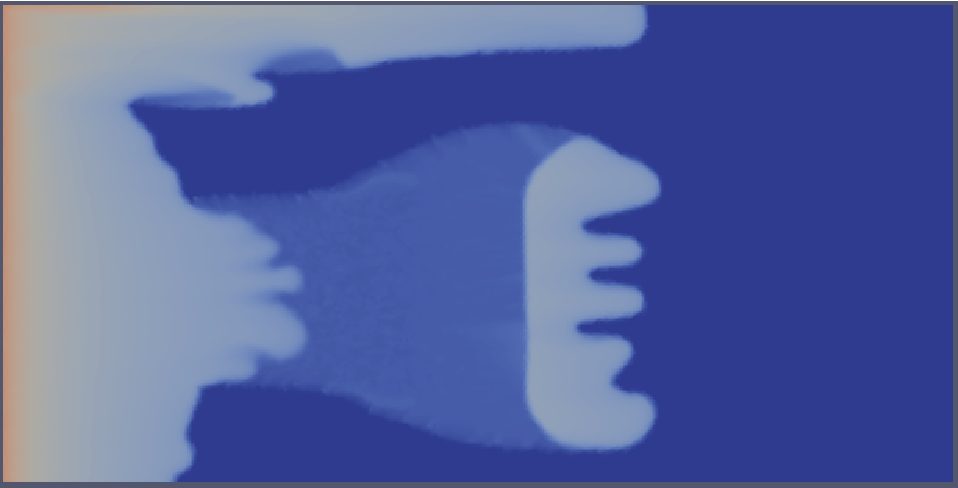
\includegraphics[width=.65\textwidth]{./Pics1/5reg_dinlet_fixed_500.pdf} 
}
\vspace{0.0cm}
\hbox{\hspace{6.5cm} (a) double inlet - fixed mesh   
}
\hbox{\hspace{3.5cm}
\includegraphics[width=.9\textwidth]{./Pics1/5reg_dinlet_adapt_500_1.pdf}
}
\vspace{0.0cm}
\hbox{\hspace{6.5cm} (b) double inlet adaptive mesh   
}
}     
\caption{For $t=5$s there is a comparison between fixed mesh(a) and adaptive mesh(b).}
\label{fig:3testcase_b}
\end{figure}
\end{landscape}
\clearpage

%%%%
%%%%  FIGURE
%%%%
\begin{landscape}
\begin{figure}[ht] 
\vbox{
\hbox{\hspace{3.5cm}
\includegraphics[width=.65\textwidth]{./Pics1/5reg_dinlet_fixed_1500.pdf} 
}
\vspace{0.0cm}
\hbox{\hspace{6.5cm} (a) double inlet - fixed mesh   
}
\hbox{\hspace{3.5cm}
\includegraphics[width=.9\textwidth]{./Pics1/5reg_dinlet_adapt_1500_1.pdf}
}
\vspace{0.0cm}
\hbox{\hspace{6.5cm} (b) double inlet adaptive mesh   
}
}     
\caption{For $t=7.5$s this is a comparison between fixed mesh(a) and adaptive mesh(b).}
\label{fig:3testcase_c}
\end{figure}
\end{landscape}
\clearpage

%%%%
%%%%  FIGURE
%%%%
\begin{landscape}
\begin{figure}[ht] 
\vbox{
\hbox{\hspace{3.5cm}
\includegraphics[width=.65\textwidth]{./Pics1/5reg_dinlet_fixed_end.pdf} 
}
\vspace{0.0cm}
\hbox{\hspace{6.5cm} (a) double inlet - fixed mesh   
}
\hbox{\hspace{3.5cm}
\includegraphics[width=.9\textwidth]{./Pics1/5reg_dinlet_adapt_end_1.pdf}
}
\vspace{0.0cm}
\hbox{\hspace{6.5cm} (b) double inlet adaptive mesh   
}
}     
\caption{This is a comparison between fixed mesh(a) and adaptive mesh(b) at the end of the simulation. For the fixed mesh at this point the maximum number of point is $13226$ while for the adaptive mesh is $7582$ and most of them are located where is needed in the domain.}
\label{fig:3testcase_d}
\end{figure}
\end{landscape}
\clearpage

%%%%
%%%%  FIGURE
%%%%
\begin{landscape}
\begin{figure}[ht] 
\vbox{
\hbox{\hspace{3.5cm}
\includegraphics[width=.8\textwidth]{./Pics1/mr100_fixed/mr100_fixed_500.pdf} 
}
\vspace{0.0cm}
\hbox{\hspace{4.0cm} (a) fixed and unstructured mesh for MR = 100 (start)   
}
\hbox{\hspace{3.5cm}
\includegraphics[width=.8\textwidth]{./Pics1/mr100_fixed/mr100_fixed_1500.pdf}
}
\vspace{0.0cm}
\hbox{\hspace{3.75cm} (b) fixed and unstructured mesh for MR = 100 (t = 1500)   
}
}     
\caption{For the case of VR=$100$ from top to bottom, the number of elements is $4680$ and fixed and unstructured mesh for the same time steps, t=$0.25$ or t=500(a), t=$0.75$ or t=1500(b). }
\label{fig:4testcase_a}
\end{figure}
\end{landscape}
\clearpage

%%%%
%%%%  FIGURE
%%%%
\begin{landscape}
\begin{figure}[ht] 
\vbox{
\hbox{\hspace{3.5cm}
\includegraphics[width=.8\textwidth]{./Pics1/mr100_fixed/mr100_fixed_3000.pdf} 
}
\vspace{0.0cm}
\hbox{\hspace{3.75cm} (c) fixed and unstructured mesh for MR = 100    
}
\hbox{\hspace{3.5cm}
\includegraphics[width=.8\textwidth]{./Pics1/mr100_fixed/mr100_fixed_end.pdf}
}
\vspace{0.0cm}
\hbox{\hspace{7.cm} (d) end of simulations     
}
}     
\caption{screenshot (c) is for t=$1.5$ sec or t=$3000$ and screenshot (d) is for t=$3.175$ sec, at the end of the simulations. }
\label{fig:4testcase_b}
\end{figure}
\end{landscape}
\clearpage


 

\end{document}
%% End of tex file.


